% Options for packages loaded elsewhere
\PassOptionsToPackage{unicode}{hyperref}
\PassOptionsToPackage{hyphens}{url}
\PassOptionsToPackage{dvipsnames,svgnames,x11names}{xcolor}
%
\documentclass[
]{article}

\usepackage{amsmath,amssymb}
\usepackage{iftex}
\ifPDFTeX
  \usepackage[T1]{fontenc}
  \usepackage[utf8]{inputenc}
  \usepackage{textcomp} % provide euro and other symbols
\else % if luatex or xetex
  \usepackage{unicode-math}
  \defaultfontfeatures{Scale=MatchLowercase}
  \defaultfontfeatures[\rmfamily]{Ligatures=TeX,Scale=1}
\fi
\usepackage{lmodern}
\ifPDFTeX\else  
    % xetex/luatex font selection
    \setmainfont[]{Times New Roman}
  \setmathfont[]{Times New Roman}
\fi
% Use upquote if available, for straight quotes in verbatim environments
\IfFileExists{upquote.sty}{\usepackage{upquote}}{}
\IfFileExists{microtype.sty}{% use microtype if available
  \usepackage[]{microtype}
  \UseMicrotypeSet[protrusion]{basicmath} % disable protrusion for tt fonts
}{}
\makeatletter
\@ifundefined{KOMAClassName}{% if non-KOMA class
  \IfFileExists{parskip.sty}{%
    \usepackage{parskip}
  }{% else
    \setlength{\parindent}{0pt}
    \setlength{\parskip}{6pt plus 2pt minus 1pt}}
}{% if KOMA class
  \KOMAoptions{parskip=half}}
\makeatother
\usepackage{xcolor}
\usepackage[margin=1in]{geometry}
\setlength{\emergencystretch}{3em} % prevent overfull lines
\setcounter{secnumdepth}{-\maxdimen} % remove section numbering
% Make \paragraph and \subparagraph free-standing
\makeatletter
\ifx\paragraph\undefined\else
  \let\oldparagraph\paragraph
  \renewcommand{\paragraph}{
    \@ifstar
      \xxxParagraphStar
      \xxxParagraphNoStar
  }
  \newcommand{\xxxParagraphStar}[1]{\oldparagraph*{#1}\mbox{}}
  \newcommand{\xxxParagraphNoStar}[1]{\oldparagraph{#1}\mbox{}}
\fi
\ifx\subparagraph\undefined\else
  \let\oldsubparagraph\subparagraph
  \renewcommand{\subparagraph}{
    \@ifstar
      \xxxSubParagraphStar
      \xxxSubParagraphNoStar
  }
  \newcommand{\xxxSubParagraphStar}[1]{\oldsubparagraph*{#1}\mbox{}}
  \newcommand{\xxxSubParagraphNoStar}[1]{\oldsubparagraph{#1}\mbox{}}
\fi
\makeatother


\providecommand{\tightlist}{%
  \setlength{\itemsep}{0pt}\setlength{\parskip}{0pt}}\usepackage{longtable,booktabs,array}
\usepackage{calc} % for calculating minipage widths
% Correct order of tables after \paragraph or \subparagraph
\usepackage{etoolbox}
\makeatletter
\patchcmd\longtable{\par}{\if@noskipsec\mbox{}\fi\par}{}{}
\makeatother
% Allow footnotes in longtable head/foot
\IfFileExists{footnotehyper.sty}{\usepackage{footnotehyper}}{\usepackage{footnote}}
\makesavenoteenv{longtable}
\usepackage{graphicx}
\makeatletter
\newsavebox\pandoc@box
\newcommand*\pandocbounded[1]{% scales image to fit in text height/width
  \sbox\pandoc@box{#1}%
  \Gscale@div\@tempa{\textheight}{\dimexpr\ht\pandoc@box+\dp\pandoc@box\relax}%
  \Gscale@div\@tempb{\linewidth}{\wd\pandoc@box}%
  \ifdim\@tempb\p@<\@tempa\p@\let\@tempa\@tempb\fi% select the smaller of both
  \ifdim\@tempa\p@<\p@\scalebox{\@tempa}{\usebox\pandoc@box}%
  \else\usebox{\pandoc@box}%
  \fi%
}
% Set default figure placement to htbp
\def\fps@figure{htbp}
\makeatother
% definitions for citeproc citations
\NewDocumentCommand\citeproctext{}{}
\NewDocumentCommand\citeproc{mm}{%
  \begingroup\def\citeproctext{#2}\cite{#1}\endgroup}
\makeatletter
 % allow citations to break across lines
 \let\@cite@ofmt\@firstofone
 % avoid brackets around text for \cite:
 \def\@biblabel#1{}
 \def\@cite#1#2{{#1\if@tempswa , #2\fi}}
\makeatother
\newlength{\cslhangindent}
\setlength{\cslhangindent}{1.5em}
\newlength{\csllabelwidth}
\setlength{\csllabelwidth}{3em}
\newenvironment{CSLReferences}[2] % #1 hanging-indent, #2 entry-spacing
 {\begin{list}{}{%
  \setlength{\itemindent}{0pt}
  \setlength{\leftmargin}{0pt}
  \setlength{\parsep}{0pt}
  % turn on hanging indent if param 1 is 1
  \ifodd #1
   \setlength{\leftmargin}{\cslhangindent}
   \setlength{\itemindent}{-1\cslhangindent}
  \fi
  % set entry spacing
  \setlength{\itemsep}{#2\baselineskip}}}
 {\end{list}}
\usepackage{calc}
\newcommand{\CSLBlock}[1]{\hfill\break\parbox[t]{\linewidth}{\strut\ignorespaces#1\strut}}
\newcommand{\CSLLeftMargin}[1]{\parbox[t]{\csllabelwidth}{\strut#1\strut}}
\newcommand{\CSLRightInline}[1]{\parbox[t]{\linewidth - \csllabelwidth}{\strut#1\strut}}
\newcommand{\CSLIndent}[1]{\hspace{\cslhangindent}#1}

\usepackage{booktabs}
\usepackage{caption}
\usepackage{longtable}
\usepackage{colortbl}
\usepackage{array}
\usepackage{anyfontsize}
\usepackage{multirow}
\makeatletter
\@ifpackageloaded{caption}{}{\usepackage{caption}}
\AtBeginDocument{%
\ifdefined\contentsname
  \renewcommand*\contentsname{Table of contents}
\else
  \newcommand\contentsname{Table of contents}
\fi
\ifdefined\listfigurename
  \renewcommand*\listfigurename{List of Figures}
\else
  \newcommand\listfigurename{List of Figures}
\fi
\ifdefined\listtablename
  \renewcommand*\listtablename{List of Tables}
\else
  \newcommand\listtablename{List of Tables}
\fi
\ifdefined\figurename
  \renewcommand*\figurename{Figure}
\else
  \newcommand\figurename{Figure}
\fi
\ifdefined\tablename
  \renewcommand*\tablename{Table}
\else
  \newcommand\tablename{Table}
\fi
}
\@ifpackageloaded{float}{}{\usepackage{float}}
\floatstyle{ruled}
\@ifundefined{c@chapter}{\newfloat{codelisting}{h}{lop}}{\newfloat{codelisting}{h}{lop}[chapter]}
\floatname{codelisting}{Listing}
\newcommand*\listoflistings{\listof{codelisting}{List of Listings}}
\makeatother
\makeatletter
\makeatother
\makeatletter
\@ifpackageloaded{caption}{}{\usepackage{caption}}
\@ifpackageloaded{subcaption}{}{\usepackage{subcaption}}
\makeatother

\usepackage{bookmark}

\IfFileExists{xurl.sty}{\usepackage{xurl}}{} % add URL line breaks if available
\urlstyle{same} % disable monospaced font for URLs
\hypersetup{
  pdftitle={Beyond the herd: Decoding individual animal behavioral narratives through data},
  pdfauthor={Kehan Sheng1, Borbala Foris1,2, Daniel M. Weary1, Marina A.G. von Keyserlingk1},
  colorlinks=true,
  linkcolor={blue},
  filecolor={Maroon},
  citecolor={Blue},
  urlcolor={Blue},
  pdfcreator={LaTeX via pandoc}}


\title{Beyond the herd: Decoding individual animal behavioral narratives
through data}
\author{Kehan Sheng\textsuperscript{1}, Borbala
Foris\textsuperscript{1,2}, Daniel M. Weary\textsuperscript{1}, Marina
A.G. von Keyserlingk\textsuperscript{1}}
\date{}

\begin{document}
\maketitle


\textsuperscript{1}Animal Welfare Program, Faculty of Land and Food
Systems, The University of British Columbia, 2357 Main Mall, Vancouver,
BC, V6T 1Z6, Canada

\textsuperscript{2}Animal Welfare Science Unit, University of Veterinary
Medicine, Veterinärpl. 1, Vienna, 1210, Austria

\textbf{Corresponding author email:} marina.vonkeyserlingk@ubc.ca

\begin{center}\rule{0.5\linewidth}{0.5pt}\end{center}

\section{1. Introduction}\label{introduction}

Cave paintings from 45,000 years ago show early depictions of humans and
pigs (\citeproc{ref-mcdermott2021}{McDermott, 2021}), providing evidence
that humans have shared a long history of caring for animals. For our
ancient ancestors, understanding animal behavior was no doubt central to
informing animal care (\citeproc{ref-breed2021}{Breed and Moore, 2021}).
This early interest in animal behaviors included observing animals'
movements, social interactions, cognition, and learning
(\citeproc{ref-breed2021}{Breed and Moore, 2021}). There is also
evidence that many ancient civilizations used changes in behavioral
signs to identify ill animals under their care
(\citeproc{ref-griffith1898}{Griffith, 1898}). By the 1800s, naturalists
like Charles Darwin were using behavioral observations to infer animals'
affective states, demonstrating that animals express emotions such as
fear, pleasure, and anger through their behavior
(\citeproc{ref-darwin1872}{Darwin, 1872};
\citeproc{ref-fraser2025}{Fraser, 2025}).

Fast forwarding to the 20th century, in the industrialized world, the
production of food from animals had intensified, largely driven by
mechanization that reducee number of people required to care for a
growing number of livestock (\citeproc{ref-rollin2011animal}{Rollin,
2011}). Although automation was integrated into many aspects of
livestock farming, the monitoring of animal health continued to rely on
the accumulated experience of human care givers through manual
behavioral observations (\citeproc{ref-hornbuckle1992}{Hornbuckle and
Morgan, 1992}). These observations focused on identifying sickness
behaviors associated with general malaise, such as reduced food and
water intake and decreased activity
(\citeproc{ref-hart1988biological}{Hart, 1988}). Veterinary medicine has
also adopted the approach of providing treatment and manage health at
the herd level rather than the individual level
(\citeproc{ref-medeiros2022historical}{Medeiros et al., 2022}). These
traditional approaches to identifying sick animals shared a common
limitation: they typically considered the behavior of animals as a
species or population rather than recognizing the importance of
individual differences.

More recently, there has been a paradigm shift toward understanding
individual differences in behavior (see
\citeproc{ref-neave2020long}{Neave et al., 2020};
\citeproc{ref-weary2009}{Weary et al., 2009}). This shift acknowledges
what individual animals housed in identical environments exhibit
remarkably different behaviors and strategies, even when healthy, due to
their distinct personalities (\citeproc{ref-carslake2022a}{Carslake et
al., 2022a}; \citeproc{ref-neave2020long}{Neave et al., 2020}). Previous
research also emphasized the need to assess animal welfare at the
individual rather than herd level, since it is individual animals, not
herds, that could suffer (\citeproc{ref-fraser2025}{Fraser, 2025}).

Recent advancement of Precision Livestock Farming (PLF) technologies
such as electronic feeders and drinkers offer new opportunities to
automatically and continuously monitor animals on individual level,
particularly behavioral and physiological measures
(\citeproc{ref-dittrich2019}{Dittrich et al., 2019}). This continuous
monitoring is especially valuable for prey species, which often hide
signs of illness when humans are present (\citeproc{ref-weary2009}{Weary
et al., 2009}). PLF has been widely promoted as tools for early disease
detection (\citeproc{ref-dittrich2019}{Dittrich et al., 2019}). However,
much of the PLF research to date has focused on between subject
comparison at the group level, such as comparing a specific behavior
between healthy and sick groups (\citeproc{ref-cramer2015}{Cramer and
Stanton, 2015}; \citeproc{ref-goharshahi2021}{Goharshahi et al., 2021}).
This population-level thinking fails to account for the substantial
individual differences in behavioral expression that is increasingly
being documented in the literature
(\citeproc{ref-carslake2022a}{Carslake et al., 2022a}). These consistent
behavioral differences across time and context reflect distinct animal
personalities (\citeproc{ref-neave2020long}{Neave et al., 2020}).

Also of interest is that as animals become sick, the magnitude and
direction of their behavioral changes vary dramatically between
individuals; a phenomenon that has been attributed to personality
differences (\citeproc{ref-setser2024a}{Setser et al., 2024a}). For
instance, when comparing lying behavior in `fearful' versus `active'
dairy calves with diarrhea, fearful calves reduced their lying bouts
while active calves increased them (\citeproc{ref-setser2024a}{Setser et
al., 2024a}). This personality-based variability extends to other
behaviors as well. Foe, a recent study found that calves differ greatly
in the consistency of their space-use behavior: some calves use a
consistent amount of space across days, while others show dramatic
day-to-day variation (\citeproc{ref-occhiuto2022}{Occhiuto et al.,
2022}). Interpreting such behavioral changes requires understanding each
animal's baseline patterns. For highly variable individuals, substantial
changes in space use may be normal, whereas for consistent individuals,
the same degree of change could signal health problems.

Although PLF has the ability to monitor animals individually, their full
potential cannot be realized if data analysis and decision-making are
made based on group-level averages. The key to effective disease
detection lies in first understanding and tracking each animal's healthy
behavioral patterns, then identifying when they deviate from their
personal baseline. Recent studies have used multi-level models to
understand individual behavioral baseline, quantify behavioral type (an
individual's average expression oain behaviors), repeatability
(consistent between-individual differences), and predictability
(individual differences in within-individual consistency) (elephants:
(\citeproc{ref-hertel2020}{Hertel et al., 2020}); dairy cows:
(\citeproc{ref-thomas2024}{Thomas et al., 2024}); dairy calves:
(\citeproc{ref-carslake2022b}{Carslake et al., 2022b};
\citeproc{ref-occhiuto2022}{Occhiuto et al., 2022})). However, existing
research has focused primarily on simple metrics such as feed or water
intake and feeding or drinking duration.

In the current study, we demonstrate that existing PLF systems can
extend beyond these basic metrics, as these technologies capture rich
data that can be used to derive novel behavioral variables. For
instance, electronic feed bins could provide data on feed bin switches
per meal as a measure of exploratory behavior
(\citeproc{ref-meagher2017}{Meagher et al., 2017}). Additionally,
agonistic interactions at feed bins can be identified when the interval
between one cow exiting and the next cow entering is exceptionally
short, suggesting that the incoming cow physically displaced or socially
threatened the departing cow (\citeproc{ref-foris2019automatic}{Foris et
al., 2019}; \citeproc{ref-huzzey2014automatic}{Huzzey et al., 2014}).
The ability to include novel behavioral measures could also
revolutionize personality assessment in farm animals
(\citeproc{ref-setser2024b}{Setser et al., 2024b}). Traditional
personality tests, which often involve isolating animals for choice and
motivation tasks (\citeproc{ref-dawkins2021}{Dawkins, 2021}), are
increasingly criticized as they may not reflect animals' natural
behavior in group settings (\citeproc{ref-biro2012}{Biro, 2012}). In
contrast, data-driven approaches using longitudinal PLF measurements
enable researchers to identify personality traits by observing animals
in their home pen environments with herd mates
(\citeproc{ref-carslake2022a}{Carslake et al., 2022a};
\citeproc{ref-setser2024b}{Setser et al., 2024b}).

In this study, we aim to:

\textbf{1. Introduce an R package for extracting behavioral variables
from electronic feeder and drinker data.} We developed the
\texttt{moo4feed} R package to enable researchers to reliably clean and
process raw electronic feeder and drinker data using distribution-based
thresholds customized to their own dataset. The package extracts both
standard feedingnd drinking measures (e.g., intake, visits, and meals)
and novel behavioral variables (e.g., non-nutritive visits, feed bin
switches per meal), revealing the rich behavioral information already
embedded within existing PLF data streams.

\textbf{2. Quantify individual-level behavioral consistency and
between-individual differences.} Using repeatability and predictability
measures, we assess which behavioral variables exhibit stable
between-individual differences and which are characterized by greater
within-individual variability, thereby identifying behaviors most
informative for characterizing individual behavioral profiles.

\textbf{3. Identify distinct behavioral profiles through cluster
analysis.} Using behaviors that exhibit consistent between-individual
differences, we group cows with similar behavioral types to reveal the
diversity of behavioral profiles present within a herd. To illustrate
the practical value of this approach, we present individual behavioral
narratives for one representative animal from each cluster,
demonstrating how data can be used to tell each animal's unique story.

This research lays the groundwork for individual-based behavioural
monitoring systems, which might improve health prediction, affective
state assessment, natural behavior monitoring, and personality
assessment.

\section{3. Methods}\label{methods}

\subsection{3.1 Animals, Housing, and Data
Collection}\label{animals-housing-and-data-collection}

Data were collected as part of a larger study described in detail by
Sheng et al. (\citeproc{ref-sheng2024redefining}{2024}). Briefly, 159
lactating Holstein dairy cows (12 primiparous, 147 multiparous; parity =
3.0 ± 1.1; mean ± SD) were enrolled over a 10-month period (July 2020 to
May 2021) at The University of British Columbia (UBC) Dairy Education
and Research Centre in Agassiz, BC, Canada. All procedures were approved
by the UBC Animal Ethics Committee (protocol A19-0299). Cows were housed
in a dynamic group of 48 in a pen equipped with 48 sand-bedded lying
stalls, 30 electronic feed bins, and 5 electronic water bins (Insentec,
Hokofarm, Emmeloord, the Netherlands). The electronic bins identified
individual cows via radio frequency identification and recorded the cow
identification, bin number, visit start and end times, and start and end
weight of the feed or water in the bin for each visit
(\citeproc{ref-chapinal2007validation}{Chapinal et al., 2007}). Cows
were milked twice daily and total mixed ration was delivered twice daily
while cows were away for milking. On average, every 16 ± 3 d, 6 ± 2 cows
were removed from the pen and replaced with new animals (i.e.,
regrouping event); individual cows remained in the trial for an average
of 86 ± 54 d.~Farm staff performed daily health checks, and a trained
observer scored locomotion weekly using a 5-level scale
(\citeproc{ref-flower2006effect}{Flower and Weary, 2006}) to identify
lame cows. A portion of the data gathered in this research was
previously published at Sheng et al.
(\citeproc{ref-sheng2024redefining}{2024}).

\subsection{3.2 Data Cleaning and
Filtering}\label{data-cleaning-and-filtering}

All data preparation and analysis were conducted using R (version 4.3.1;
R Core Team (\citeproc{ref-R-base}{2025})). To ensure that the data we
analyze reflect the behavioural baseline patterns of cows when they are
healthy and not in estrus, we applied stricter data cleaning and
filtering criteria that extended beyond the data cleaning procedure
described in our previous work (\citeproc{ref-sheng2024redefining}{Sheng
et al., 2024}). Starting from 14,728 cow-days across 159 cows and 306 d,
exclusions were applied at two levels. At the individ level, data were
removed for specific cows on days affected by:

\begin{enumerate}
\def\labelenumi{(\arabic{enumi})}
\item
  health events, including illness episodes when cows were moved to the
  hospital pen and when cows received veterinary treatment while
  remaining in the pen (e.g., mastitis, fever, injury), with a buffer
  period around each event (7 days before and 7 days after the recorded
  events) to account for potential behavioural changes during the
  prodromal and recovery periods (16 cows across 120 days, 197
  cow-days).
\item
  lameness, defined as two consecutive weekly locomotion scores
  \textgreater= 3 (\citeproc{ref-eriksson2020effects}{Eriksson et al.,
  2020}; \citeproc{ref-flower2006effect}{Flower and Weary, 2006}), with
  all days during the lame period removed until the cow was scored as
  sound again, plus a 7-d buffer before lameness onset (48 cows across
  227 days, 679 cow-days).
\item
  the first and last day each cow was present in the group, as data on
  these days would be incomplete (159 cows across 43 days, 285
  cow-days).
\item
  days when farm staff recorded interference with individual cows due to
  lose of ear tags, hoof trimming or other routine husbandry procedures,
  as these events may temporarily alter behaviour through handling
  stress or cows being away from the Insentec bins for extended period
  of times (9 cows across 22 days, 24 cow-days).
\item
  days when cows were not confirmed pregnant, as reproductive status
  (e.g., bred, fresh, open) may influence behaviour through oestrous
  cycling and associated hormonal fluctuations; only cow-days where the
  reproductive status was recorded as pregnant were retained (87 cows
  across 207 days, 2,695 cow-days removed).
\end{enumerate}

At the herd level, data were removed for all cows on days affected by:

\begin{enumerate}
\def\labelenumi{(\arabic{enumi})}
\item
  estrus events, as any cow in heat potentially disturb the behaviour of
  all other cows in the group (55 estrus events, 2,381 cow-days).
\item
  technical disruptions to the Insentec recording system, including
  equipment breakdowns, compressor failures, power outages, missing
  data, and severe weather events that compromised bin function (28 d,
  1,281 cow-days).
\item
  regrouping events when the herd dynamics is destabilized (16 events,
  674 cow-days).
\end{enumerate}

After filtering, 107 cows with sufficient data across 207 days (10-130
days of observation per cow), 6226 unique cow-days were retained.

\subsection{3.3 Behavioral Variable
Extraction}\label{behavioral-variable-extraction}

To process the raw feeding and drinking data collected by the Insentec
system and extract meaningful behavioral variables, we developed an
open-source R package called moo4feed
(\textless www.skysheng.io/moo4feed/\textgreater). This package provides
a standardized workflow for handling electronic feed and water bin data
and supports a broad range of analyses. The functionality used in this
study spans five key areas: (1) data processing, configuration, and
quality control; (2) agonistic replacement detection; (3) non-nutritive
visit detection; (4) feed availability estimation; and (5) meal
clustering and analysis. Note that moo4feed includes additional
variables and functionalities beyond the scope of this paper, such as
pairwise synchronicity analysis.

\textbf{Data Processing, Configuration and Quality Control.} The package
includes a global configuration system that allows users to tailor data
processing to their specific farm setup. Users can customize settings
such as column name mappings, time zones, bin identifiers, and the
physical layout of bins in the barn, making the tool adaptable to a wide
range of data formats and facility designs. The package also includes an
automated module for handling daylight saving time (DST) transitions
across North American time zones. For any given year and time zone, this
module identifies the exact dates and times of spring-forward and
fall-back transitions. During fall-back transitions (when clocks move
back one hour, causing chronological order of visits within the repeated
hour to be ambiguous), the package removes all visits from the
duplicated hour, since it is not possible to determine the true
chronological order, and adjusts subsequent timestamps accordingly.
During spring-forward transitions (when clocks move forward by one
hour), visit timestamps are shifted forward by one hour for the
remainder of the day. This automated handling ensures temporal
consistency across all visit records without manual correction.
Additional details on the reproducible workflow are provided in Section
3.5.

The first processing step converts raw visit data into a standardized
format, with each record capturing the cow's identity, the bin number,
the start and end times of the visit, and the start and end weight of
the feed or water in the bin. Only days for which both feeder and
drinker data files were available were retained for analysis. Feed and
water visit data then go through automated quality control check, which
includes multiple validation steps: checking whether the expected number
of cows was present each day to warn users when cows went missing or
lost their ear tags, detecting and correcting double detections
(instances where the same cow was recorded at two different bins
simultaneously, which indicates potential bin malfunction), flagging
records with negative durations, intakes, or weight measurements,
identifying abnormally large single-visit feed or water intakes,
flagging cows that did not feed or drink after noon (which may indicate
a lost ear tag or illness), and flagging bins with unusually low traffic
or no visits (which may indicate equipment malfunction). Visits with
implausibly long durations were flagged using customizable thresholds
(set to \textgreater2,000 s for feed bins and \textgreater1,800 s for
water bins in this study), as were visits with unrealistically large
single-visit intake amounts (\textgreater8 kg for feed; \textgreater30 L
for water) or excessively high intake rates (\textgreater0.008 kg/s for
feed; \textgreater0.35 L/s for water). Days on which a cow recorded
fewer than 10 visits were flagged as potentially incomplete, typically
due to technical issues such as bin breakdowns, and cows with abnormally
low or high daily feed intake (\textless35 or \textgreater75 kg/d) or
daily water intake (\textless60 or \textgreater180 L/d) were also
flagged. This validation procedure functions as a warning system rather
than a data filter. All flagged records are retained in the dataset, and
researchers receive a summary report to support informed, daily
decision-making about data quality on farm.

Following this initial quality control, additional outlier detection was
performed using a k-nearest neighbor (KNN) algorithm
(\citeproc{ref-malini2017analysis}{Malini and Pushpa, 2017}) applied to
scaled visit duration, intake, and intake rate. Unlike the traditional
approach of removing data points beyond three standard deviations (SD)
from the mean, which applies rigid rectangular cutoffs, the KNN method
operates in multidimensional space, considering the relationships among
all three variables at once. This enables the detection of visits that
appear plausible on any single dimension but are implausible in
combination. The KNN algorithm compares each data point to its nearest
neighbors and flags those that are unusually distant from their local
cluster. Users can adjust the number of neighbors (k = 50 in this
study), the percentile threshold for flagging (0.04\% of feed visits and
0.1\% of water visits were flagged as outliers in this study), and the
relative scaling of each variable to control how aggressively outliers
are detected. The package also provides visualization tools that allow
users to inspect flagged outliers in two-dimensional plots (e.g., intake
versus duration, or intake rate versus intake) before deciding whether
to remove them.

After cleaning, the feed and water datasets are combined, and daily
summaries of basic feeding and drinking metrics are calculated. This
step yields six conventional behavioral variables: (i) total daily feed
intake (kg), (ii) total daily feeding duration (s), (iii) total number
of feeding visits per day, (iv) total daily water intake (L), (v) total
daily drinking duration (s), and (vi) total number of drinking visits
per day.

\textbf{Agonistic Replacement Detection.} Replacements at the feed bins
were identified using a validated algorithm following the method
described by Huzzey et al. (\citeproc{ref-huzzey2014automatic}{2014})
and Foris et al. (\citeproc{ref-foris2019automatic}{2019}). A
replacement was recorded when one cow (the actor) entered a feed bin
within 26 seconds of another cow (the reactor) leaving that same bin,
serving as a proxy for the actor physically pushing the reactor away
from the bin. Replacement events were discarded if the presumed actor
was already feeding at a different bin at the time the reactor exited,
as this would indicate that the reactor likely left voluntarily rather
than being displaced (\citeproc{ref-foris2019automatic}{Foris et al.,
2019}). Daily agonistic behavior was summarized into two variables:
(vii) total number of times the focal cow acted as the actor (displacing
another cow from a bin) per day, and (viii) total number of times the
focal cow acted as the reactor (being displaced from a bin) per day.

\textbf{Non-nutritive Visit Detection.} A visit was classified as
non-nutritive if the cow's measured intake did not exceed the
calibration error of the Insentec system (0.5 kg), meaning the cow
visited a bin that contained feed but did not eat anything. This yielded
one daily-level variable: (ix) total number of non-nutritive feed visits
per cow per day.

\textbf{Feed Availability Estimation.} Feed delivery events were
automatically identified when a bin's start weight increased by at least
5 kg (threshold is customizable) between consecutive visits, with
deliveries to multiple bins grouped together if they occurred within one
hour. This approach allows users to track both the frequency of feeding
events throughout the day and the exact amount of feed added to each
individual bin during every delivery. By combining this with visit-level
bin weight data, it becomes possible to estimate how much feed remained
in each bin at the precise moment a cow arrived, enabling us to identify
cows that consistently are disadvantaged and end up accessing bins only
after much of the fresh feed has already been consumed. For each feeding
visit, the proportion of feed remaining in the bin at the time of the
cow's arrival was estimated. This produced one variable: (x) median
proportion of feed remaining in the bin at visit start (\%), calculated
as the daily median across all of a cow's visits to all the feed bins.
The median was used in place of the mean as the measure of central
tendency, given that the underlying distributions of these variables are
often skewed and do not conform to normality assumptions. This variable
indicates whether a cow consistently arrived at bins with ample feed or
tended to access nearly depleted bins, helping flag individuals that may
be socially disadvantaged and forced to eat leftover feed.

\textbf{Meal Clustering and Analysis.} Individual feed bin visits were
grouped into meals using a density-based clustering algorithm: DBSCAN
(\citeproc{ref-khan2014dbscan}{Khan et al., 2014}), which identifies
clusters of temporally close visits based on two parameters: a maximum
time gap between consecutive visits within a meal (the meal criterion),
and a minimum number of visits required to form a meal. The meal
criterion was determined in a data-driven manner rather than using an
arbitrary fixed interval (e.g., 60 or 90 minutes), which fails to
account for differences among farms, data collection methods, and
individual animals' differences.

To derive the meal criterion, we first extracted all inter-visit
intervals (i.e., the time gaps between consecutive feed bin visits from
the same animal) pooled across all animals and days. Because these gap
times are highly right-skewed (most gaps are short, but a few are very
long), a log transformation was applied before fitting a two-component
Gaussian Mixture Model (GMM) (\citeproc{ref-tolkamp1998satiety}{Tolkamp
et al., 1998}). The two components naturally capture two distinct
populations of gaps: short within-meal pauses and longer between-meal
gaps. The meal criterion was then set to the point where the two fitted
distributions intersect. The moo4feed package visualizes the gap
distribution and the fitted mixture components so users can confirm the
two populations are well separated for their own data. As a simpler
alternative, the package also supports a percentile-based approach,
where the meal criterion is set to a user-specified percentile of the
gap distribution (e.g., the 90th percentile). The meal criterion can be
derived at three levels of granularity: a single universal threshold
pooled across all animals and days, an animal-specific threshold applied
consistently across all days, or a threshold estimated separately for
each animal on each day. In this study, we used a single pooled
criterion derived from the GMM method. Meals were required to contain a
minimum of two visits. The DBSCAN algorithm then assigned each visit to
a meal cluster or flagged it as an isolated, unclustered visit. Timeline
visualizations of the resulting meal clusters were generated for each
animal on each day to allow visual inspection of the clustering results.

Once visits were grouped into meals, meal-level variables were computed
by aggregating visit-level data within each meal and then summarizing
across all meals within each cow-day. This step yielded six meal-level
variables: (xi) total number of meals per day, (xii) median meal
duration (s), (xiii) median number of visits per meal, (xiv) median feed
intake per meal (kg), (xv) median percentage of time spent feeding per
meal, calculated as the proportion of the meal's total duration during
which the cow was actively occupying a feed bin (total visit time ÷ meal
duration × 100\%), and (xvi) median number of non-nutritive visits per
meal.

In total, 16 behavioral variables were included in the statistical
analyses described in Section 3.4: six basic daily feeding and drinking
variables (i--vi), two daily agonistic variables (vii--viii), one
non-nutritive visit variable (ix), one feed availability variable (x),
and six meal-level variables (xi--xvi).

\subsection{3.4 Statistical Analysis}\label{statistical-analysis}

We used Bayesian mixed-effects models to quantify repeatability and
predictability. All models were fitted using the brms R package
(\citeproc{ref-burkner2017brms}{Bürkner, 2017}), which implements
Bayesian regression models via the Stan programming language.

\textbf{Variable distribution assessment.} Before fitting any models, we
examined the distribution of each behavioral variable by plotting
histograms on both the raw and log-transformed scale. For each variable,
we computed skewness, the proportion of zero values, and conducted
Shapiro-Wilk normality test. This informed the likelihood family
selected for each Bayesian model: variables with approximately symmetric
distributions were modeled using a Gaussian likelihood (feed intake,
feeding duration, water intake, median percentage of time spent feeding
per meal, median proportion of feed remaining when cow starts feeding),
while strongly right-skewed variables were modeled using a lognormal
likelihood (number of feeding visits, drinking duration, number of
drinking visits, total meals, median meal duration, median visits per
meal, median feed intake per meal, number of non-nutritive visits,
median non-nutritive visits per meal, total actor events, and total
reactor events). Three variables modeled with a lognormal likelihood
(median non-nutritive visits per meal, total actor events, and total
reactor events) were shifted by adding a constant of 1 prior to model
fitting, given that the lognormal distribution requires strictly
positive values and each of these variables contained zero values.
Posterior estimates for these variables were shifted back to the
original scale for interpretation.

\textbf{Repeatability.} For each of the 16 behavioral variables, a
Bayesian mixed model was fitted:

\[
\text{response} \sim \text{DIM} + \text{parity} + \text{THI}_{\text{mean}} + \text{poly}(\text{month},\, 2) + (1 \mid \text{cow})
\]

where DIM (days in milk), parity, and mean daily THI were fixed effects
controlling for changes in physiological state and thermal environment,
a second-degree polynomial of calendar month captured seasonal trends,
and cow identity was a random intercept. Default brms priors were used.
MCMC sampling used 4 chains with 1,000 warmup iterations; total
iterations ranged from 6,000 to 17,000 per variable to ensure
convergence.

Between-individual variation was quantified using two metrics derived
from posterior draws: repeatability \textbf{(R)} and the coefficient of
individual variation \textbf{(CVi)} (\citeproc{ref-hertel2020}{Hertel et
al., 2020}). R is the proportion of total variance attributable to
between-cow differences:

\[
R = \frac{\text{var.cow}}{\text{var.cow} + \text{var.res}}
\]

where \(\text{var.cow}\) is the posterior variance of the cow-level
random intercept and \(\text{var.res}\) is the residual variance. R is
thus confounded by the within-individual variance. A high value of R
could mean cows differ a lot from each other, or simply mean that each
cow is very consistent within herself. To resolve this ambiguity, we
also computed CVi, which calculates between-individual spread relative
to the population mean, independently of within-individual consistency:

\[
\text{CVi} = \frac{\sqrt{\text{var.cow}}}{\bar{y}}
\]

where \(\bar{y}\) is the mean of the response variable. For lognormal
models, CVi was instead computed as \(\sqrt{\exp(\text{var.cow}) - 1}\)
to place the estimate on the original data scale. CVi is interpretable
across behaviors with different units and facilitates comparison across
studies. Model convergence was assessed via R-hat (\textless{} 1.01),
Bulk- and Tail-Effective Sample Size (ESS), trace plots, and posterior
predictive checks. Individual-level posterior distributions were
visualized using ridge plots ordered by each cow's posterior mean.

\textbf{Predictability.} Within-individual variance was quantified using
a double hierarchical generalized linear model (DHGLM) implemented in
brms. In addition to modeling the mean response, brms allows a variance
structure to also be imposed on the residual variance (i.e.,
within-individual variance). Each DHGLM extended the repeatability model
by adding a cow-level random effect to the residual variance,
partitioning it per individual so that cows with high residual variance
are identified as more unpredictable than cows with low residual
variance:

\[
\text{sigma} \sim (1 \mid \text{cow})
\]

Population-level predictability was summarized using two metrics derived
from the posterior SD of the cow-level random effect in the sigma
sub-model (\(\text{sd.sigma.cow}\)). The residual intra-individual
variability \textbf{(rIIV)} captures how much cows differ from one
another in their within-individual consistency
(\citeproc{ref-hertel2020}{Hertel et al., 2020}):

\[
\text{rIIV} = \exp(\text{sd.sigma.cow})^2
\]

We also computed the coefficient of variation of predictability
\textbf{(CVP)}, which can be used to compare predictability across
different behavioural traits and studies, independent of the scale of
the trait:

\[
\text{CVP} = \sqrt{\exp(\text{sd.sigma.cow}^2) - 1}
\]

A high CVP value means that cows differ considerably from each other in
how consistent their day-to-day behavior is: for example, some cows may
eat nearly the same amount of feed every day, while others fluctuate
substantially. A low CVP value means that cows are similar to each other
in their level of day-to-day consistency: whether that means all cows
are highly consistent, or all cows are highly variable, there is little
difference between individuals in their within-individual consistency.
MCMC sampling settings were identical to those used for the
repeatability models.

Behavioral variables that showed both high CVi and low CVP are the best
candidates for individual profiling, as these are behaviors that differ
meaningfully across individuals and remain stable within individuals
over time.

\textbf{Behavioral variable clustering.} To organize the 16 behavioral
variables by how informative they are for individual profiling, we
applied k-means clustering (k = 3, 50 random starts) to the posterior
mean CVi and R values for each variable, after scaling both dimensions.
The number of clusters (k = 3) was determined by researcher judgment
based on visual inspection of the CVi and R distributions. All variables
have low predictaibility values, thus measures of predictability were
not used in behavioral variable clustering. The three clusters were
labeled by descending R and CVi: Cluster 1 (high R, high CVi: traits in
which cows differ substantially in their average levels relative to the
trait mean, and those individual differences are consistent over time);
Cluster 2 (high R, low CVi: traits in which individual differences are
consistent over time, but the variation among cows is small relative to
the trait mean); and Cluster 3 (low R, low CVi: traits in which cows
show little variation relative to the trait mean, and what little
variation exists is not consistent over time). We used only the
variables in Cluster 1 for the downstream cow clustering, as they are
the most informative for individual cow profiling.

\textbf{Individual-level behavioral profiles.} For each cow and each
behavioral variable in Cluster 1, we extracted the individual intercept
from the posterior distribution: the population intercept plus each
cow's random effect (back-transformed to the original scale for
lognormal models). This represents a cow's average behavioral type
(i.e., a cow's typical expression of their behavior).

\textbf{PCA and cow clustering using k-means.} To synthesize the
multi-dimensional behavioral profiles into a small number of
interpretable dimensions and identify distinct cow types, we applied
principal component analysis (PCA) with varimax rotation
(\citeproc{ref-budaev2010using}{Budaev, 2010}) to the matrix of
individual intercepts for the Cluster 1 variables (one row per cow, one
column per variable). The number of components retained was chosen to
explain at least 80\% of the cumulative variance.

Following PCA, cows were grouped into behavioral types by applying
k-means clustering to the retained rotated component scores. The optimal
number of clusters \(k\) was determined using the silhouette method,
evaluated across 100 independent runs with different random seeds, each
using 100 random centroid initializations for stability. For each run,
the value of \(k\) yielding the highest mean silhouette score was
selected, and the \(k\) chosen most frequently across all seeds was used
for the final clustering.

The silhouette score quantifies how well each data point fits its
assigned cluster relative to neighboring clusters. For each cow \(i\)
belonging to cluster \(C_i\), we first compute \(a(i)\), the mean
distance from cow \(i\) to all other cows within the same cluster:

\[
a(i) = \frac{1}{|C_i| - 1} \sum_{j \in C_i,\, j \neq i} d(i, j)
\]

where \(|C_i|\) is the number of cows in cluster \(C_i\) and \(d(i, j)\)
is the Euclidean distance between cows \(i\) and \(j\). A smaller
\(a(i)\) indicates that cow \(i\) is tightly grouped with its cluster
members.

We then compute \(b(i)\), the mean distance from cow \(i\) to all cows
in the nearest neighboring cluster (i.e., the cluster \(C \neq C_i\)
that minimizes the expression below):

\[
b(i) = \min_{C \neq C_i} \frac{1}{|C|} \sum_{h \in C} d(i, h)
\]

A larger \(b(i)\) indicates that cow \(i\) is well-separated from
neighboring clusters. The silhouette score for cow \(i\) is then defined
as:

\[
s(i) = \begin{cases}
  1 - \dfrac{a(i)}{b(i)}, & \text{if } a(i) < b(i) \\[6pt]
  0, & \text{if } a(i) = b(i) \\[6pt]
  \dfrac{b(i)}{a(i)} - 1, & \text{if } a(i) > b(i)
\end{cases}
\]

Values of \(s(i)\) range from \(-1\) to \(1\), where values close to
\(1\) indicate that the cow is well-matched to its own cluster and
clearly separated from others, values near \(0\) indicate borderline
assignment, and negative values suggest possible misclassification.

The mean silhouette score \(\bar{s}\) across all cows serves as an
overall measure of cluster quality, reflecting both within-cluster
cohesion and between-cluster separation. The resulting clusters were
visualized using component score biplots and an interactive 3D scatter
plot for exploration of cow clusters across three principal components.

\subsection{3.5 Reproducible Data Science Workflow and
Software}\label{reproducible-data-science-workflow-and-software}

To support full transparency and reproducibility, all data processing,
variable extraction, and analytical steps were implemented in the
moo4feed R package \textless www.skysheng.io/moo4feed/\textgreater,
which is publicly available with detailed tutorials. The functions
implemented in this R package have been thoroughly tested with 96\% code
coverage (code coverage report:
\url{https://app.codecov.io/gh/skysheng7/moo4feed}). This R package
enables future researchers to replicate our variable extraction pipeline
on their own datasets and to extend the approach to additional
behavioral measures. The source code and example data included in the R
package is hosted on GitHub:
\url{https://github.com/skysheng7/moo4feed.git}. We used the newly
developed R package to extract the behavioral variables described in
Section 3.3 and conduct all statistical analyses described in Section
3.4, data and code for all the data analysis are available at:
\url{https://github.com/skysheng7/competition_dominance_analysis.git}.
We have also used Borealis to archive the R package at:
\url{https://doi.org/10.5683/SP3/LF4DRO} and data analysis code at:
\url{https://doi.org/10.5683/SP3/K6J350}.

\section{4. Results}\label{results}

\subsection{4.1 Between-Individual Variation: Repeatability and
CVi}\label{between-individual-variation-repeatability-and-cvi}

Throughout this section, all repeatability and predictability measures
(R, CVi, CVP, and rIIV) are reported as posterior means followed by
their 95\% credible intervals (CrIs) in square brackets.

Because R is confounded by within-individual variance (Section 3.4), we
use the coefficient of individual variation (CVi) as the primary metric
for comparing the magnitude of between-individual differences across the
16 behavioral variables, and we report R alongside CVi as a reference
for how reliably those differences persist from day to day
(Table~\ref{tbl-rep-pred}, Figure~\ref{fig-rep-cvp-scatter}).

Among all variables, the total number of non-nutritive visits showed the
largest relative between-individual spread (CVi = 0.53 {[}0.45,
0.61{]}), meaning that on average, cows differ from one another by more
than half the population mean in how often they visit a feed bin without
eating. The total number of actor events (CVi = 0.47 {[}0.40, 0.54{]})
and the median number of non-nutritive visits per meal (CVi = 0.44
{[}0.38, 0.51{]}) were also highly variable across individuals,
indicating that agonistic and non-nutritive visiting tendencies are
among the most individually distinguishing behaviors in this herd. At
the other end of the spectrum, the percentage of meal time spent
actively feeding (CVi = 0.09 {[}0.08, 0.10{]}) and daily feed intake
(CVi = 0.10 {[}0.08, 0.11{]}) showed the smallest relative spread,
meaning cows are nearly indistinguishable from one another on these
dimensions.

Repeatability (R) provides complementary but not redundant information.
Daily water drinking duration had the highest R (0.74 {[}0.69, 0.79{]}),
followed by daily feeding visits (R = 0.68 {[}0.62, 0.74{]}) and the
total number of non-nutritive visits (R = 0.64 {[}0.58, 0.70{]}). The
lowest R values were observed for the median proportion of feed
remaining when a cow arrived at a bin (R = 0.21 {[}0.16, 0.26{]}),
median feed intake per meal (R = 0.29 {[}0.23, 0.36{]}), and median meal
duration (R = 0.31 {[}0.25, 0.38{]}).

As anticipated in Section 3.4, R and CVi do not always rank traits the
same way, and the divergences are informative. The clearest example is
the median percentage of meal time spent feeding, which has a moderately
high R (0.59 {[}0.53, 0.66{]}) but the lowest CVi of all 16 variables
(0.09 {[}0.08, 0.10{]}). This is the signature of a trait where
within-individual variance is small --- cows are each very consistent
from day to day --- but cows are also nearly identical to each other, so
R is inflated by low noise rather than by real individual differences.
The opposite pattern is seen for agonistic behavior: total actor events
have a moderate R (0.50 {[}0.43, 0.57{]}) but one of the highest CVi
values (0.47 {[}0.40, 0.54{]}), and total reactor events show the same
pattern (R = 0.44 {[}0.37, 0.51{]}; CVi = 0.38 {[}0.32, 0.43{]}). Here,
cows genuinely differ from one another by a large margin, but their
day-to-day variability is also substantial, so R is moderate despite
large between-individual spread. Variables ranked near the top on both R
and CVi --- notably the total number of non-nutritive visits, water
drinking duration, and the median number of non-nutritive visits per
meal --- represent the most useful candidates for individual profiling,
since cows both differ meaningfully from one another and behave
consistently enough for those differences to be detectable from repeated
observations.

\begin{table}

\caption{\label{tbl-rep-pred}Repeatability (R), coefficient of
individual variation (CVi), coefficient of variation of predictability
(CVP), and residual intra-individual variability (rIIV) for the 16
behavioral variables. Values are posterior means with 95\% credible
intervals in brackets. Cell color encodes the posterior mean within each
metric (darker = higher). Rows are grouped by behavioral category.}

\centering{

\fontsize{12.0pt}{14.0pt}\selectfont
\begin{tabular*}{\linewidth}{@{\extracolsep{\fill}}lcccc}
\toprule
{\bfseries \cellcolor[HTML]{1F3A93}{\textcolor[HTML]{FFFFFF}{Variable}}} & {\bfseries \cellcolor[HTML]{1F3A93}{\textcolor[HTML]{FFFFFF}{\textbf{R} {[}95\% CI{]}}}} & {\bfseries \cellcolor[HTML]{1F3A93}{\textcolor[HTML]{FFFFFF}{\textbf{CVi} {[}95\% CI{]}}}} & {\bfseries \cellcolor[HTML]{1F3A93}{\textcolor[HTML]{FFFFFF}{\textbf{CVP} {[}95\% CI{]}}}} & {\bfseries \cellcolor[HTML]{1F3A93}{\textcolor[HTML]{FFFFFF}{\textbf{rIIV} {[}95\% CI{]}}}} \\ 
\midrule\addlinespace[2.5pt]
\multicolumn{5}{l}{{\bfseries \textcolor[HTML]{1F3A93}{Feeding}}} \\[2.5pt] 
\midrule\addlinespace[2.5pt]
{Daily feed intake} & {\cellcolor[HTML]{A3C0A1}{\textcolor[HTML]{000000}{0.39 [0.32, 0.46]}}} & {\cellcolor[HTML]{E0E5F3}{\textcolor[HTML]{000000}{0.10 [0.08, 0.11]}}} & {\cellcolor[HTML]{BF360C}{\textcolor[HTML]{FFFFFF}{0.22 [0.18, 0.26]}}} & {\cellcolor[HTML]{4A148C}{\textcolor[HTML]{FFFFFF}{1.55 [1.44, 1.68]}}} \\ 
{Daily feeding duration} & {\cellcolor[HTML]{628F60}{\textcolor[HTML]{FFFFFF}{0.56 [0.49, 0.63]}}} & {\cellcolor[HTML]{CFD1E8}{\textcolor[HTML]{000000}{0.14 [0.12, 0.15]}}} & {\cellcolor[HTML]{DF7D57}{\textcolor[HTML]{FFFFFF}{0.17 [0.14, 0.21]}}} & {\cellcolor[HTML]{8F65B5}{\textcolor[HTML]{FFFFFF}{1.41 [1.32, 1.50]}}} \\ 
{Daily feeding visits} & {\cellcolor[HTML]{376F37}{\textcolor[HTML]{FFFFFF}{0.68 [0.62, 0.74]}}} & {\cellcolor[HTML]{8D86BD}{\textcolor[HTML]{FFFFFF}{0.29 [0.25, 0.34]}}} & {\cellcolor[HTML]{DF7E57}{\textcolor[HTML]{FFFFFF}{0.17 [0.14, 0.20]}}} & {\cellcolor[HTML]{8F65B5}{\textcolor[HTML]{FFFFFF}{1.41 [1.32, 1.50]}}} \\ 
{Median \% feed remaining} & {\cellcolor[HTML]{E8F5E9}{\textcolor[HTML]{000000}{0.21 [0.16, 0.26]}}} & {\cellcolor[HTML]{D3D6EB}{\textcolor[HTML]{000000}{0.13 [0.11, 0.15]}}} & {\cellcolor[HTML]{E07F59}{\textcolor[HTML]{FFFFFF}{0.17 [0.14, 0.20]}}} & {\cellcolor[HTML]{9067B6}{\textcolor[HTML]{FFFFFF}{1.40 [1.31, 1.50]}}} \\ 
\midrule\addlinespace[2.5pt]
\multicolumn{5}{l}{{\bfseries \textcolor[HTML]{1F3A93}{Drinking}}} \\[2.5pt] 
\midrule\addlinespace[2.5pt]
{Daily water intake} & {\cellcolor[HTML]{669263}{\textcolor[HTML]{FFFFFF}{0.55 [0.48, 0.62]}}} & {\cellcolor[HTML]{CFD1E8}{\textcolor[HTML]{000000}{0.14 [0.12, 0.15]}}} & {\cellcolor[HTML]{DD7851}{\textcolor[HTML]{FFFFFF}{0.18 [0.14, 0.21]}}} & {\cellcolor[HTML]{8A5FB2}{\textcolor[HTML]{FFFFFF}{1.42 [1.33, 1.51]}}} \\ 
{Daily drinking duration} & {\cellcolor[HTML]{1B5E20}{\textcolor[HTML]{FFFFFF}{0.74 [0.69, 0.79]}}} & {\cellcolor[HTML]{6159A2}{\textcolor[HTML]{FFFFFF}{0.39 [0.34, 0.45]}}} & {\cellcolor[HTML]{D15D34}{\textcolor[HTML]{FFFFFF}{0.20 [0.16, 0.23]}}} & {\cellcolor[HTML]{7041A2}{\textcolor[HTML]{FFFFFF}{1.48 [1.38, 1.58]}}} \\ 
{Daily drinking visits} & {\cellcolor[HTML]{669263}{\textcolor[HTML]{FFFFFF}{0.55 [0.48, 0.62]}}} & {\cellcolor[HTML]{918AC0}{\textcolor[HTML]{FFFFFF}{0.28 [0.24, 0.32]}}} & {\cellcolor[HTML]{E1825C}{\textcolor[HTML]{000000}{0.17 [0.14, 0.20]}}} & {\cellcolor[HTML]{936AB7}{\textcolor[HTML]{FFFFFF}{1.40 [1.31, 1.49]}}} \\ 
\midrule\addlinespace[2.5pt]
\multicolumn{5}{l}{{\bfseries \textcolor[HTML]{1F3A93}{Meal patterns}}} \\[2.5pt] 
\midrule\addlinespace[2.5pt]
{Total meals} & {\cellcolor[HTML]{A4C1A2}{\textcolor[HTML]{000000}{0.38 [0.32, 0.45]}}} & {\cellcolor[HTML]{C8C9E4}{\textcolor[HTML]{000000}{0.15 [0.13, 0.17]}}} & {\cellcolor[HTML]{F0AD8C}{\textcolor[HTML]{000000}{0.14 [0.10, 0.17]}}} & {\cellcolor[HTML]{BA99D0}{\textcolor[HTML]{000000}{1.31 [1.23, 1.40]}}} \\ 
{Median meal duration} & {\cellcolor[HTML]{BED5BD}{\textcolor[HTML]{000000}{0.31 [0.25, 0.38]}}} & {\cellcolor[HTML]{BBB9DB}{\textcolor[HTML]{000000}{0.18 [0.16, 0.21]}}} & {\cellcolor[HTML]{FAD2B9}{\textcolor[HTML]{000000}{0.11 [0.07, 0.14]}}} & {\cellcolor[HTML]{D9C3E4}{\textcolor[HTML]{000000}{1.23 [1.16, 1.31]}}} \\ 
{Median visits per meal} & {\cellcolor[HTML]{729B6F}{\textcolor[HTML]{FFFFFF}{0.52 [0.45, 0.59]}}} & {\cellcolor[HTML]{7D75B3}{\textcolor[HTML]{FFFFFF}{0.33 [0.28, 0.38]}}} & {\cellcolor[HTML]{FCDDC5}{\textcolor[HTML]{000000}{0.10 [0.07, 0.12]}}} & {\cellcolor[HTML]{E2CEEA}{\textcolor[HTML]{000000}{1.21 [1.15, 1.28]}}} \\ 
{Median intake per meal} & {\cellcolor[HTML]{C7DCC6}{\textcolor[HTML]{000000}{0.29 [0.23, 0.36]}}} & {\cellcolor[HTML]{BDBCDC}{\textcolor[HTML]{000000}{0.18 [0.15, 0.21]}}} & {\cellcolor[HTML]{C84B22}{\textcolor[HTML]{FFFFFF}{0.21 [0.17, 0.25]}}} & {\cellcolor[HTML]{5E2C97}{\textcolor[HTML]{FFFFFF}{1.51 [1.40, 1.63]}}} \\ 
{Median feeding \% per meal} & {\cellcolor[HTML]{568654}{\textcolor[HTML]{FFFFFF}{0.59 [0.53, 0.66]}}} & {\cellcolor[HTML]{E3E8F5}{\textcolor[HTML]{000000}{0.09 [0.08, 0.10]}}} & {\cellcolor[HTML]{C84921}{\textcolor[HTML]{FFFFFF}{0.21 [0.17, 0.25]}}} & {\cellcolor[HTML]{5D2A96}{\textcolor[HTML]{FFFFFF}{1.52 [1.40, 1.63]}}} \\ 
\midrule\addlinespace[2.5pt]
\multicolumn{5}{l}{{\bfseries \textcolor[HTML]{1F3A93}{Non-nutritive behavior}}} \\[2.5pt] 
\midrule\addlinespace[2.5pt]
{Non-nutritive visits} & {\cellcolor[HTML]{447943}{\textcolor[HTML]{FFFFFF}{0.64 [0.58, 0.70]}}} & {\cellcolor[HTML]{1A237E}{\textcolor[HTML]{FFFFFF}{0.53 [0.45, 0.61]}}} & {\cellcolor[HTML]{CA4F26}{\textcolor[HTML]{FFFFFF}{0.21 [0.17, 0.24]}}} & {\cellcolor[HTML]{62319A}{\textcolor[HTML]{FFFFFF}{1.51 [1.40, 1.62]}}} \\ 
{Median non-nutritive per meal} & {\cellcolor[HTML]{649161}{\textcolor[HTML]{FFFFFF}{0.56 [0.49, 0.62]}}} & {\cellcolor[HTML]{4A4495}{\textcolor[HTML]{FFFFFF}{0.44 [0.38, 0.51]}}} & {\cellcolor[HTML]{FFF3E0}{\textcolor[HTML]{000000}{0.08 [0.05, 0.11]}}} & {\cellcolor[HTML]{F3E5F5}{\textcolor[HTML]{000000}{1.17 [1.11, 1.24]}}} \\ 
\midrule\addlinespace[2.5pt]
\multicolumn{5}{l}{{\bfseries \textcolor[HTML]{1F3A93}{Social dominance}}} \\[2.5pt] 
\midrule\addlinespace[2.5pt]
{Total actor events} & {\cellcolor[HTML]{79A076}{\textcolor[HTML]{FFFFFF}{0.50 [0.43, 0.57]}}} & {\cellcolor[HTML]{3F3B8E}{\textcolor[HTML]{FFFFFF}{0.47 [0.40, 0.54]}}} & {\cellcolor[HTML]{C44219}{\textcolor[HTML]{FFFFFF}{0.22 [0.18, 0.25]}}} & {\cellcolor[HTML]{562292}{\textcolor[HTML]{FFFFFF}{1.53 [1.42, 1.65]}}} \\ 
{Total reactor events} & {\cellcolor[HTML]{90B28D}{\textcolor[HTML]{000000}{0.44 [0.37, 0.51]}}} & {\cellcolor[HTML]{6961A7}{\textcolor[HTML]{FFFFFF}{0.38 [0.32, 0.43]}}} & {\cellcolor[HTML]{E99673}{\textcolor[HTML]{000000}{0.15 [0.12, 0.19]}}} & {\cellcolor[HTML]{A681C3}{\textcolor[HTML]{FFFFFF}{1.35 [1.27, 1.44]}}} \\ 
\bottomrule
\end{tabular*}
\begin{minipage}{\linewidth}
\vspace{.05em}
\emph{R} = repeatability; \emph{CVi} = individual coefficient of variation; \emph{CVP} = coefficient of variation of predictability; \emph{rIIV} = residual intra-individual variability. Darker fills indicate larger posterior means within each metric.\\
\end{minipage}

}

\end{table}%

\phantomsection\label{cell-fig-rep-cvp-scatter}
\begin{figure}[H]

\centering{

\pandocbounded{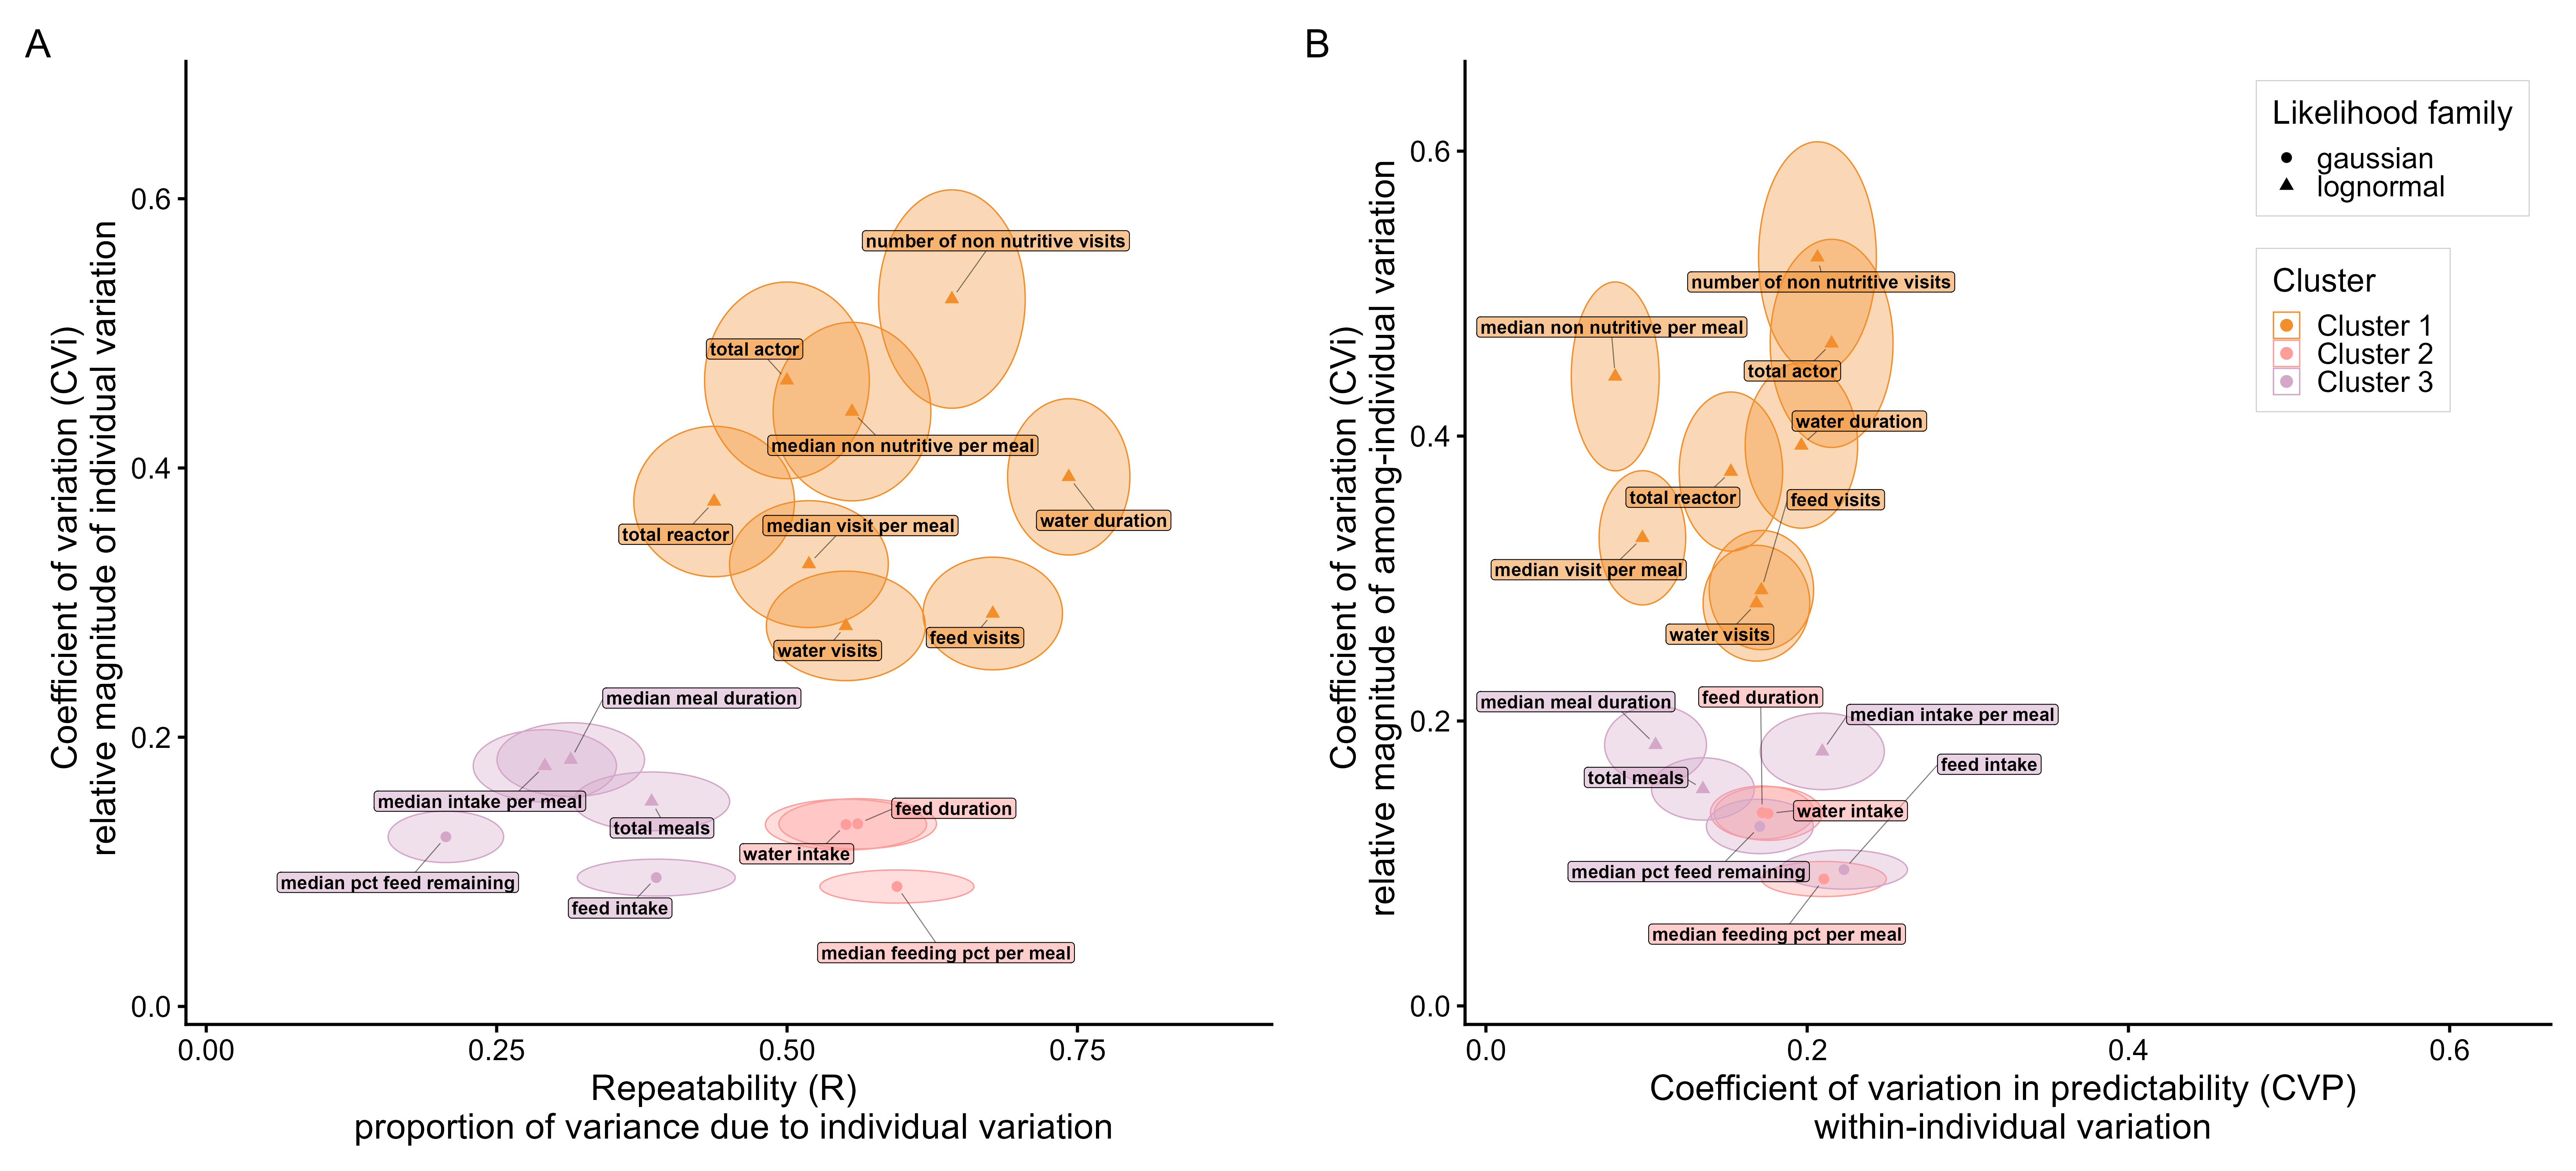
\includegraphics[keepaspectratio]{results/14_individual_traits/ellipse_scatter_grid_AB.png}}

}

\caption{\label{fig-rep-cvp-scatter}Between- and within-individual
variation in the 16 behavioral variables. (A) Repeatability (R) vs
coefficient of individual variation (CVi). (B) Coefficient of variation
of predictability (CVP) vs CVi. Each point is a behavioral variable;
ellipses show 95\% credible intervals on both axes. Points are coloured
by the 3-cluster k-means solution of Section 4.3 (Cluster 1 = high R,
high CVi; Cluster 2 = high R, low CVi; Cluster 3 = low R, low CVi).
Point shape distinguishes the likelihood family used for the mixed
model.}

\end{figure}%

\subsection{4.2 Within-Individual Variation:
Predictability}\label{within-individual-variation-predictability}

For the same reason that R is not directly comparable across traits,
residual intra-individual variability (rIIV) also depends on the scale
of each variable and is not directly interpretable across behaviors. We
therefore use the coefficient of variation of predictability (CVP) as
the primary metric for cross-trait comparisons of day-to-day
consistency, and report rIIV alongside as a reference.

Variables related to within-meal structure were the most predictable.
The median number of non-nutritive visits per meal (CVP = 0.08 {[}0.05,
0.11{]}), median visits per meal (CVP = 0.10 {[}0.07, 0.12{]}), and
median meal duration (CVP = 0.11 {[}0.07, 0.14{]}) had the lowest CVP
values, meaning individual cows expressed these behaviors at a similar
level from day to day, and cows differed little from one another in how
predictable they were. In contrast, daily feed intake (CVP = 0.22
{[}0.18, 0.26{]}), total actor events (CVP = 0.22 {[}0.18, 0.25{]}), and
the median percentage of meal time spent feeding (CVP = 0.21 {[}0.17,
0.25{]}) had the highest CVP, indicating greater individual variation in
day-to-day consistency: some cows were much more consistent than others
in these behaviors. All 16 variables had rIIV values greater than 1
(Table~\ref{tbl-rep-pred}), confirming that individual cows differ from
one another not only in their average behavioral expression but also in
how predictably they behave.

The right panel of Figure~\ref{fig-rep-cvp-scatter} shows that CVP and
CVi are largely decoupled: high between-individual spread does not
guarantee high predictability, nor vice versa. The variables most useful
for profiling (Section 4.3) occupy the high-CVi / moderate-CVP region
--- cows differ substantially from each other on these traits, and
day-to-day behavior is consistent enough for those differences to be
reliably estimated.

\subsection{4.3 Classifying Behavioral Variables by Profiling
Potential}\label{classifying-behavioral-variables-by-profiling-potential}

K-means clustering of the 16 variables based on their R and CVi values
identified three groups that differ in how useful they are for
distinguishing individuals (Figure~\ref{fig-rep-cvp-scatter}, left
panel).

\textbf{Cluster 1 --- high R, high CVi} contained 8 variables: number of
non nutritive visits, total actor, median non nutritive per meal, water
duration, total reactor, median visit per meal, feed visits, water
visits. These variables show the strongest individual-level signatures
--- cows not only behave consistently over time (high R) but also differ
substantially from one another (high CVi). These are the most
informative variables for building behavioral profiles.

\textbf{Cluster 2 --- high R, low CVi} contained 3 variables: feed
duration, water intake, median feeding pct per meal. Cows are consistent
in these behaviors over time, but all cows tend to express them at
similar levels, limiting their power to distinguish individuals from one
another.

\textbf{Cluster 3 --- low R, low CVi} contained 5 variables: median meal
duration, median intake per meal, total meals, median pct feed
remaining, feed intake. These behaviors are neither particularly
consistent within individuals nor particularly variable across them,
suggesting they are more strongly driven by daily environmental factors
(e.g., feed availability, group dynamics) than by stable individual
traits.

\subsection{4.4 Identifying Cow Types via
PCA}\label{identifying-cow-types-via-pca}

We applied PCA with varimax rotation to the intercepts of the 8 Cluster
1 variables (one row per cow, one column per variable). 3 components
were retained to meet the ≥80\% cumulative-variance criterion, together
explaining 86.1\% of the total variance (Table~\ref{tbl-pca-loadings}).
RC1 explained the largest share of variance (51.6\%), driven primarily
by non-nutritive visiting behavior and within-meal visit patterns. RC2
explained 21.3\% of variance and was most strongly associated with
drinking patterns. RC3 captured the remaining variance, primarily
related to agonistic behavior (actor and reactor events).

\begin{table}

\caption{\label{tbl-pca-loadings}Varimax-rotated PCA loadings for the 8
Cluster-1 intercept variables. Values with magnitude \textgreater{} 0.5
indicate primary drivers of each component and are the basis for
component interpretation.}

\centering{

\fontsize{12.0pt}{14.0pt}\selectfont
\begin{tabular*}{\linewidth}{@{\extracolsep{\fill}}lrrr}
\toprule
{\bfseries \cellcolor[HTML]{1F3A93}{\textcolor[HTML]{FFFFFF}{Variable}}} & {\bfseries \cellcolor[HTML]{1F3A93}{\textcolor[HTML]{FFFFFF}{RC1}}} & {\bfseries \cellcolor[HTML]{1F3A93}{\textcolor[HTML]{FFFFFF}{RC2}}} & {\bfseries \cellcolor[HTML]{1F3A93}{\textcolor[HTML]{FFFFFF}{RC3}}} \\ 
\midrule\addlinespace[2.5pt]
{number of non nutritive visits} & {0.96} & {0.02} & {0.06} \\ 
{total actor} & {0.51} & {0.30} & {-0.57} \\ 
{median non nutritive per meal} & {0.97} & {-0.01} & {0.07} \\ 
{water duration} & {-0.08} & {0.89} & {-0.17} \\ 
{total reactor} & {0.36} & {0.16} & {0.82} \\ 
{median visit per meal} & {0.94} & {-0.04} & {0.08} \\ 
{feed visits} & {0.96} & {0.05} & {0.07} \\ 
{water visits} & {0.08} & {0.91} & {0.21} \\ 
\bottomrule
\end{tabular*}

}

\end{table}%

\begin{figure}

\begin{minipage}{0.50\linewidth}

\centering{

\pandocbounded{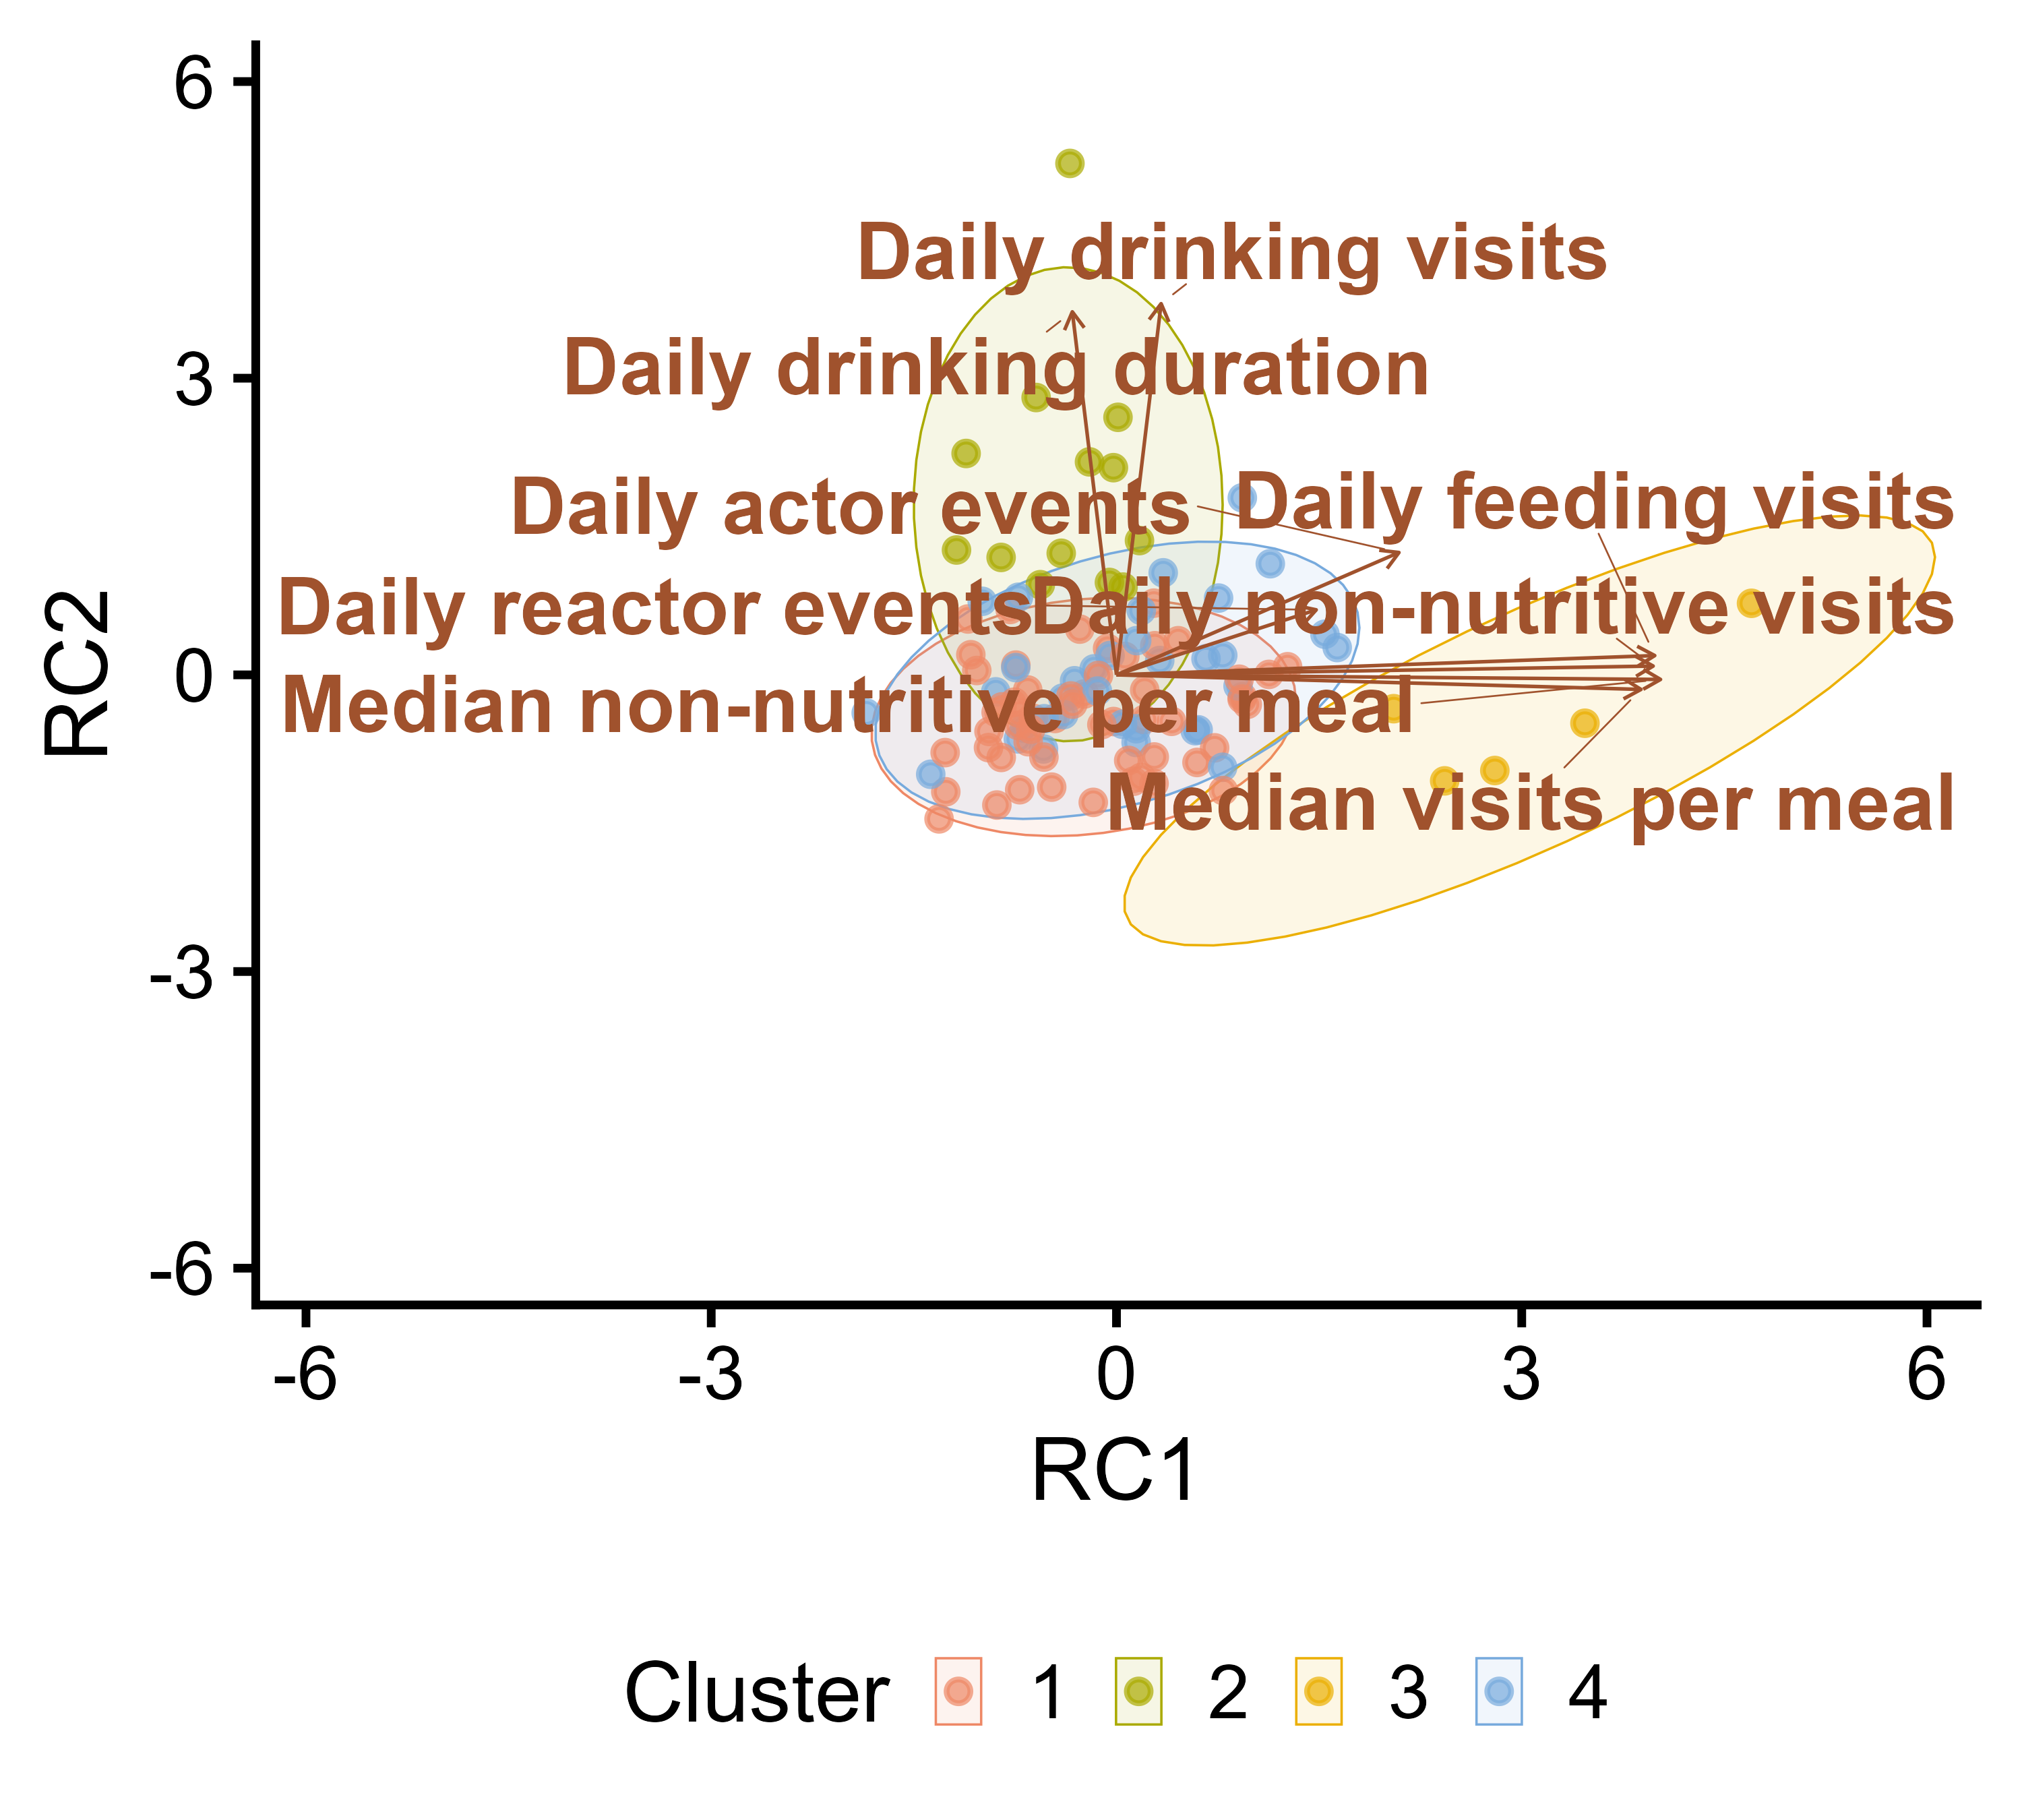
\includegraphics[keepaspectratio]{results/15_pca_clustering/pca_M3_c1_int_biplot_clusters_rc1_rc2.png}}

}

\subcaption{\label{fig-pca-biplots-1}RC1 vs RC2}

\end{minipage}%
%
\begin{minipage}{0.50\linewidth}

\centering{

\pandocbounded{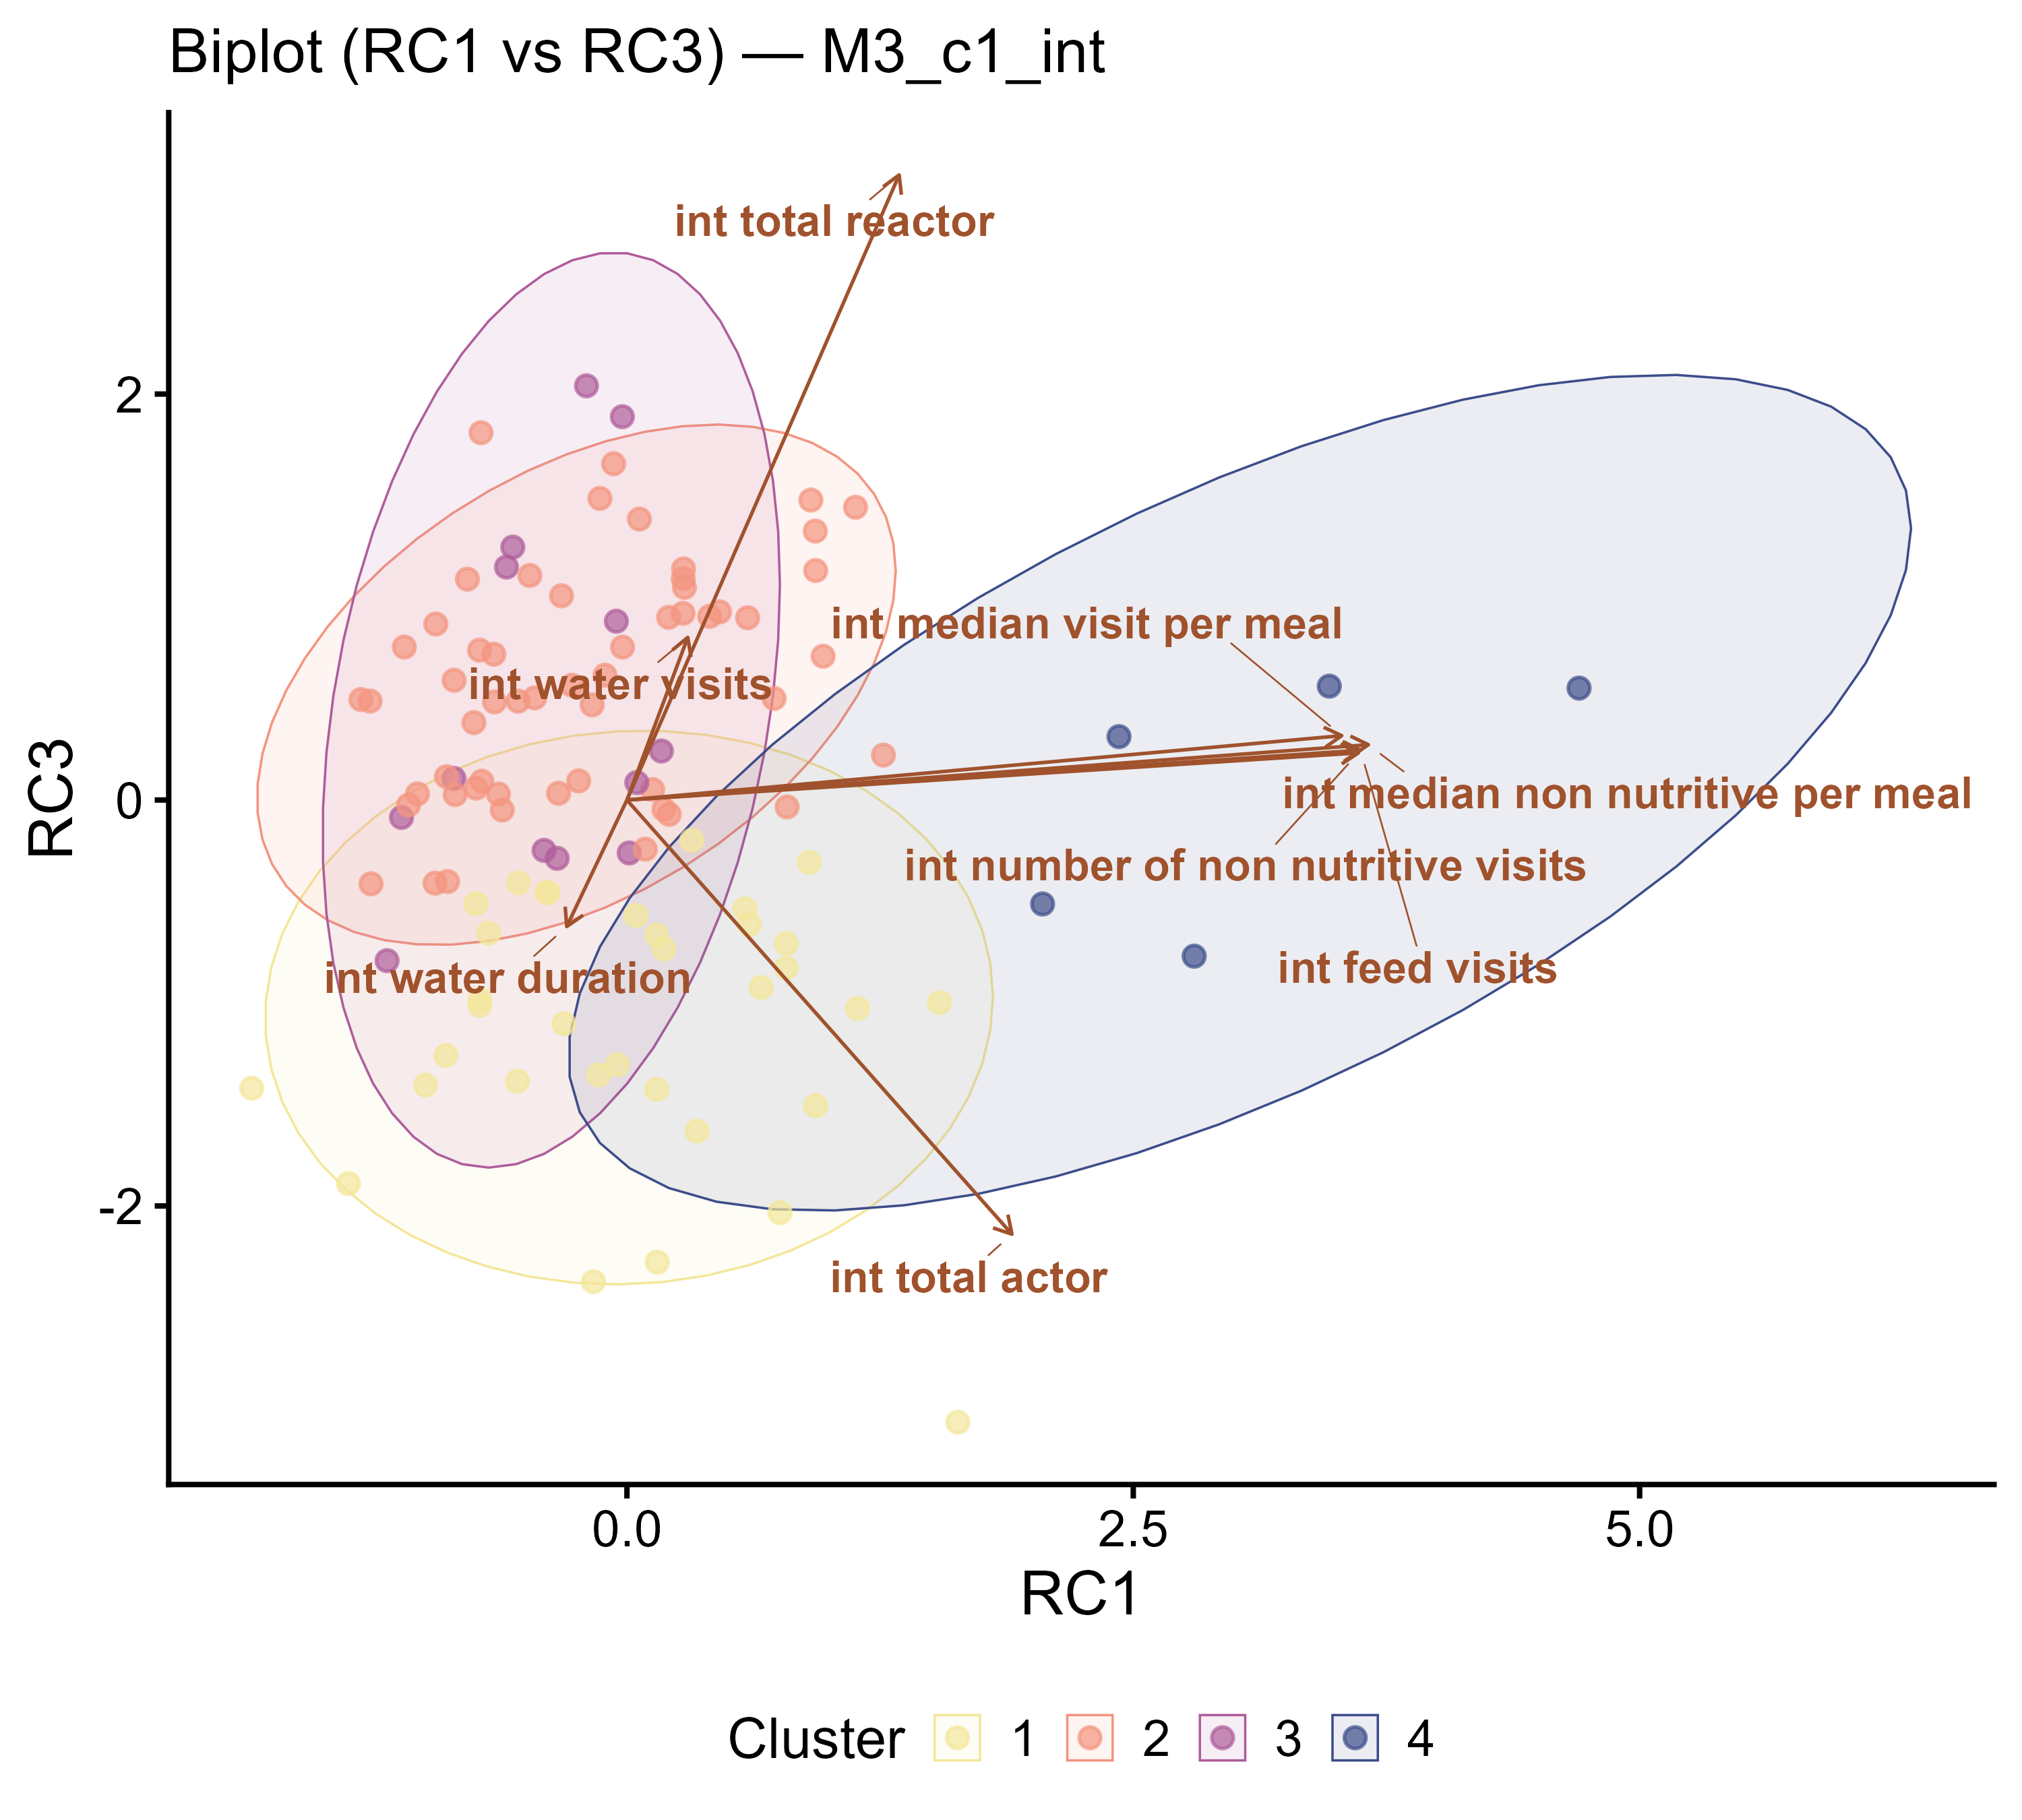
\includegraphics[keepaspectratio]{results/15_pca_clustering/pca_M3_c1_int_biplot_clusters_rc1_rc3.png}}

}

\subcaption{\label{fig-pca-biplots-2}RC1 vs RC3}

\end{minipage}%

\caption{\label{fig-pca-biplots}PCA biplots using the intercepts of
Cluster-1 variables (Method M3). Left: RC1 vs RC2. Right: RC1 vs RC3.
Each point is a cow, coloured by k-means cluster assignment; arrows
represent variable loadings scaled to the score space. Ellipses show
95\% confidence regions around each cluster centroid.}

\end{figure}%

K-means clustering on the retained component scores, with \(k\) selected
by the silhouette method, identified k = 4 as the optimal number of cow
clusters. This solution was entirely stable across all 100 random seed
replicates (100/100 seeds selected k = 4). The mean silhouette width of
the final clustering was 0.30, indicating reasonably well-defined
groupings. The 4 clusters were markedly unequal in size: one large
cluster contained 55 cows (\textasciitilde51\% of the herd), a second
contained 34 cows (\textasciitilde32\%), a third contained 13 cows
(\textasciitilde12\%), and a fourth contained only 5 cows
(\textasciitilde5\%). The smaller clusters represent cows with more
extreme or atypical behavioral profiles relative to the herd majority.
An interactive 3D visualization of cow positions in RC1--RC3 space,
colored by cluster assignment, is available at
\url{https://www.skysheng.io/moo4feed_decoding_animal/}.

\subsection{References}\label{references}

\phantomsection\label{refs}
\begin{CSLReferences}{1}{0}
\bibitem[\citeproctext]{ref-biro2012}
Biro, P.A., 2012. Do rapid assays predict repeatability in labile
(behavioural) traits? Animal Behaviour 83, 1295--1300.

\bibitem[\citeproctext]{ref-breed2021}
Breed, M.D., Moore, J., 2021. Animal behavior. Academic Press.

\bibitem[\citeproctext]{ref-budaev2010using}
Budaev, S.V., 2010. Using principal components and factor analysis in
animal behaviour research: Caveats and guidelines. Ethology 116,
472--480.

\bibitem[\citeproctext]{ref-burkner2017brms}
Bürkner, P.-C., 2017. Brms: An r package for bayesian multilevel models
using stan. Journal of statistical software 80, 1--28.

\bibitem[\citeproctext]{ref-carslake2022a}
Carslake, C., Occhiuto, F., Vázquez-Diosdado, J.A., Kaler, J., 2022a.
Indication of a personality trait in dairy calves and its link to weight
gain through automatically collected feeding behaviours. Scientific
Reports 12, 19425.

\bibitem[\citeproctext]{ref-carslake2022b}
Carslake, C., Occhiuto, F., Vázquez-Diosdado, J.A., Kaler, J., 2022b.
Repeatability and predictability of calf feeding behaviors---quantifying
between-and within-individual variation for precision livestock farming.
Frontiers in Veterinary Science 9, 827124.

\bibitem[\citeproctext]{ref-chapinal2007validation}
Chapinal, N., Veira, D., Weary, D., Von Keyserlingk, M., 2007.
Validation of a system for monitoring individual feeding and drinking
behavior and intake in group-housed cattle. Journal of dairy science 90,
5732--5736.

\bibitem[\citeproctext]{ref-cramer2015}
Cramer, M., Stanton, A., 2015. Associations between health status and
the probability of approaching a novel object or stationary human in
preweaned group-housed dairy calves. Journal of Dairy Science 98,
7298--7308.

\bibitem[\citeproctext]{ref-darwin1872}
Darwin, C., 1872. The expression of the emotions in man and animals
(republished in 1965). University of Chicago Press 10, 10001--000.

\bibitem[\citeproctext]{ref-dawkins2021}
Dawkins, M.S., 2021. The science of animal welfare: Understanding what
animals want. Oxford University Press.

\bibitem[\citeproctext]{ref-dittrich2019}
Dittrich, I., Gertz, M., Krieter, J., 2019. Alterations in sick dairy
cows' daily behavioural patterns. Heliyon 5.

\bibitem[\citeproctext]{ref-eriksson2020effects}
Eriksson, H.K., Daros, R.R., Keyserlingk, M.A. von, Weary, D.M., 2020.
Effects of case definition and assessment frequency on lameness
incidence estimates. Journal of dairy science 103, 638--648.

\bibitem[\citeproctext]{ref-flower2006effect}
Flower, F., Weary, D., 2006. Effect of hoof pathologies on subjective
assessments of dairy cow gait. Journal of dairy science 89, 139--146.

\bibitem[\citeproctext]{ref-foris2019automatic}
Foris, B., Thompson, A., Von Keyserlingk, M., Melzer, N., Weary, D.,
2019. Automatic detection of feeding-and drinking-related agonistic
behavior and dominance in dairy cows. Journal of dairy science 102,
9176--9186.

\bibitem[\citeproctext]{ref-fraser2025}
Fraser, D., 2025. Two paradigms of research and their influence on the
study of animal behaviour. Applied Animal Behaviour Science 284, 106550.

\bibitem[\citeproctext]{ref-goharshahi2021}
Goharshahi, M., Azizzadeh, M., Lidauer, L., Steininger, A., Kickinger,
F., Öhlschuster, M., Auer, W., Klein-Jöbstl, D., Drillich, M., Iwersen,
M., 2021. Monitoring selected behaviors of calves by use of an
ear-attached accelerometer for detecting early indicators of diarrhea.
Journal of Dairy Science 104, 6013--6019.

\bibitem[\citeproctext]{ref-griffith1898}
Griffith, F.L., 1898. Hieratic papyri from kahun and gurob:(principally
of the middle kingdom). B. Quaritch.

\bibitem[\citeproctext]{ref-hart1988biological}
Hart, B.L., 1988. Biological basis of the behavior of sick animals.
Neuroscience \& Biobehavioral Reviews 12, 123--137.

\bibitem[\citeproctext]{ref-hertel2020}
Hertel, A.G., Niemelä, P.T., Dingemanse, N.J., Mueller, T., 2020. A
guide for studying among-individual behavioral variation from movement
data in the wild. Movement ecology 8, 30.

\bibitem[\citeproctext]{ref-hornbuckle1992}
Hornbuckle, W., Morgan, R., 1992. General physical examination of the
cat and dog. Handbook of small animal practice. 2nd ed. New York:
Churchill Livingstone 3.

\bibitem[\citeproctext]{ref-huzzey2014automatic}
Huzzey, J., Weary, D., Tiau, B., Von Keyserlingk, M., 2014. Automatic
detection of social competition using an electronic feeding system.
Journal of dairy science 97, 2953--2958.

\bibitem[\citeproctext]{ref-khan2014dbscan}
Khan, K., Rehman, S.U., Aziz, K., Fong, S., Sarasvady, S., 2014. DBSCAN:
Past, present and future, in: The Fifth International Conference on the
Applications of Digital Information and Web Technologies (ICADIWT 2014).
IEEE, pp. 232--238.

\bibitem[\citeproctext]{ref-malini2017analysis}
Malini, N., Pushpa, M., 2017. Analysis on credit card fraud
identification techniques based on KNN and outlier detection, in: 2017
Third International Conference on Advances in Electrical, Electronics,
Information, Communication and Bio-Informatics (AEEICB). IEEE, pp.
255--258.

\bibitem[\citeproctext]{ref-mcdermott2021}
McDermott, A., 2021. News feature: What was the first "art"? How would
we know? Recently discovered cave paintings and bone carvings offer new
perspectives on long-held questions about art's origins-not to mention
the nature of art itself. Proceedings of the National Academy of
Sciences of the United States of America 118, e2117561118.
\url{https://doi.org/10.1073/pnas.2117561118}

\bibitem[\citeproctext]{ref-meagher2017}
Meagher, R.K., Weary, D.M., Keyserlingk, M.A. von, 2017. Some like it
varied: Individual differences in preference for feed variety in dairy
heifers. Applied Animal Behaviour Science 195, 8--14.

\bibitem[\citeproctext]{ref-medeiros2022historical}
Medeiros, I., Fernandez-Novo, A., Astiz, S., Simões, J., 2022.
Historical evolution of cattle management and herd health of dairy farms
in OECD countries. Veterinary sciences 9, 125.

\bibitem[\citeproctext]{ref-neave2020long}
Neave, H.W., Costa, J.H., Weary, D.M., Von Keyserlingk, M.A., 2020.
Long-term consistency of personality traits of cattle. Royal Society
open science 7.

\bibitem[\citeproctext]{ref-occhiuto2022}
Occhiuto, F., Vázquez-Diosdado, J.A., Carslake, C., Kaler, J., 2022.
Personality and predictability in farmed calves using movement and
space-use behaviours quantified by ultra-wideband sensors. Royal Society
Open Science 9, 212019.

\bibitem[\citeproctext]{ref-R-base}
R Core Team, 2025. \href{https://www.R-project.org/}{R: A language and
environment for statistical computing}. R Foundation for Statistical
Computing, Vienna, Austria.

\bibitem[\citeproctext]{ref-rollin2011animal}
Rollin, B.E., 2011. Animal rights as a mainstream phenomenon. Animals 1,
102--115.

\bibitem[\citeproctext]{ref-setser2024a}
Setser, M.W., Neave, H., Costa, J., 2024a. Are you ready for a
challenge? Personality traits influence dairy calves' responses to
disease, pain, and nutritional challenges. Journal of Dairy Science 107,
9821--9838.

\bibitem[\citeproctext]{ref-setser2024b}
Setser, M.W., Neave, H., Costa, J., 2024b. Individuality of calves:
Linking personality traits to feeding and activity daily patterns
measured by precision livestock technology. Journal of Dairy Science
107, 3235--3251.

\bibitem[\citeproctext]{ref-sheng2024redefining}
Sheng, K., Foris, B., Krahn, J., Weary, D.M., Keyserlingk, M.A. von,
2024. Redefining dominance calculation: Increased competition flattens
the dominance hierarchy in dairy cows. Journal of Dairy Science 107,
7286--7298.

\bibitem[\citeproctext]{ref-thomas2024}
Thomas, M., Occhiuto, F., Green, M., Vázquez-Diosdado, J.A., Kaler, J.,
2024. Repeatability and predictability of lying and feeding behaviours
in dairy cattle. Preventive Veterinary Medicine 233, 106357.

\bibitem[\citeproctext]{ref-tolkamp1998satiety}
Tolkamp, B., Allcroft, D., Austin, E., Nielsen, B.L., Kyriazakis, I.,
1998. Satiety splits feeding behaviour into bouts. Journal of
Theoretical Biology 194, 235--250.

\bibitem[\citeproctext]{ref-weary2009}
Weary, D., Huzzey, J., Von Keyserlingk, M., 2009. Board-invited review:
Using behavior to predict and identify ill health in animals. Journal of
animal science 87, 770--777.

\end{CSLReferences}




\end{document}
